
\section{Ángulos}



Un ángulo es un concepto abstracto que podemos llevar a la realidad para así describirlo mejor.

Un ángulo se define sobre una superficie plana y consiste en dos \emph{semirectas}, $\calL$, $\calL'$ que nacen de un punto común $S$, y lo denotamos por $\angle(\calL S\calL')$.

\begin{center}
\begin{tikzpicture}
  \draw[arrows=->,color=blue] (-3,3) -- ++(1,2) node[above] {$\calL$};
  \coordinate[label=left:$S$] (S) at (-3,3);
  \draw[arrows=->,color=red] (-3,3) -- ++(2,0) node[below] {$\calL'$};

  \draw[arrows=->,color=blue] (0,5) -- ++(0,-2) node[right] {$\calL_1$};
  \coordinate[label=left:$A$] (Sa) at (0,5);
  \draw[arrows=->,color=red] (0,5) -- ++(2,-1) node[below] {$\calL_1'$};

  \draw[arrows=->,color=red] (3,0) -- ++(-1,2) node[above] {$\calL_2'$};
  \coordinate[label=right:$B$] (B) at (3,0);
  \draw[arrows=->,color=blue] (3,0) -- ++(-2,0) node[left] {$\calL_2$};

  \draw[arrows=->,color=blue] (6,2) -- ++(-2,0) node[above] {$\calL_3$};
  \coordinate[label=below:$C$] (C) at (6,2);
  \draw[arrows=->,color=red] (6,2) -- ++(2,1) node[below] {$\calL_3'$};



\end{tikzpicture}
\end{center}

Sin embargo rotaciones y traslaciones de un ángulo dado se considerarán \emph{equivalentes}.

Así, los ángulos $\angle(\calL S \calL')$ y $\angle(\calL_2 B\calL_2')$ son equivalentes, pues rotando $\calL$ y $\calL'$ hacia la derecha y trasladando ambas del punto $S$ al punto $B$ coinciden con $\calL_2$ y $\calL_2'$ respectivamente.
Mientras que  el ángulo $\angle(\calL_3 C\calL_3')$ no es equivalente a ninguno de la figura.

De igual manera, el ángulo $\angle(\calL_1 A\calL_1')$ se considera no equivalente, ya que para hacerlo coincidir con alguno de los otros, sería necesario aplicarle una reflexión, lo cual implica ``dar vuelta'' la figura pasando por fuera del plano, y eso no se considera permitido en el presente contexto.
Podemos decir eso sí, que $\angle(\calL_1' A\calL_1)$ si es equivalente a $\angle(\calL S \calL')$.

Esto nos dice que en la definición de un ángulo, el orden en el que se especifican las semirectas es muy importante y si uno lo cambia, los ángulos dejan de ser equivalentes.



Distinguimos 3 ángulos particulares.

\begin{tikzpicture}
  \node at (0,3) {Ángulo nulo:};
  \draw[arrows=->,color=blue] (2,3) --  ++(2,1) node[above] {$\calL$};
  \coordinate[label=below:$S$] (E) at (2,3);
  \draw[arrows=->,color=red] (2,3) -- ++(2,1) node[below] {$\calL'$};  
  
  \node at (10,3) {Ángulo pleno o extendido:};
  \draw[arrows=->,color=blue] (14,3) -- ++(-2,1) node[above] {$\calL$};
  \coordinate[label=below:$S$] (F) at (14,3);
  \draw[arrows=->,color=red] (14,3) -- ++(2,-1) node[below] {$\calL''$};  
  
  \node at (0,0) {Ángulo recto:};
  \draw[arrows=->,color=blue] (2,0) -- ++(2,-2) node[above] {$\calL$};
  \coordinate[label=left:$S$] (G) at (2,0);
  \draw[arrows=->,color=red] (2,0) -- ++(2,2) node[below] {$\mathcal{R}$};
  \draw (2.2,-0.2)--(2.4,0) -- (2.2,0.2);
\end{tikzpicture}

\begin{itemize}
\item El \emph{ángulo nulo} $\angle(\calL S\calL')$ es aquel en que las dos semirectas son iguales: $\calL=\calL'$.
\item El \emph{ángulo pleno} $\angle(\calL S\calL')$ es aquel en que una semirecta es la opuesta de la otra: $\calL$ y$\calL'$ son las dos mitades de una misma recta.
  \item Un \emph{ángulo recto} es un ángulo que divide al ángulo pleno en dos ángulos equivalentes, es decir, es un ángulo $\angle(\calL S\mathcal{R})$ tal que si $\calL'$ es la opuesta de $\calL$, entonces los ángulos $\angle(\calL S\mathcal{R})$ y $\angle(\mathcal{R} S\calL')$ son equivalentes. El ángulo recto siempre se identificará con un cuadradito.
\end{itemize}

\begin{center}
\begin{tikzpicture}
  \draw[arrows=->,color=green!50!blue] (2,0) -- ++(-2,2) node[above] {$\calL'$};
  \draw (1.8,0.2)--(2,0.4) -- (2.2,0.2);
  \draw[arrows=->,color=blue] (2,0) -- ++(2,-2) node[above] {$\calL$};
  \coordinate[label=left:$S$] (G) at (2,0);
  \draw[arrows=->,color=red] (2,0) -- ++(2,2) node[below] {$\mathcal{R}$};
  \draw (2.2,-0.2)--(2.4,0) -- (2.2,0.2);
\end{tikzpicture}
\end{center}


\subsection{Medida de un ángulo}

Para medir ángulos necesitamos algún \emph{estándar}, lo más natural es considerar una medida que sea proporcional al sector que el ángulo ocupa dentro de una circunferencia de centro $S$.

Así, si asignamos una medida de $180^\circ$ al ángulo pleno, el ángulo recto debe medir $90^\circ$ ya que divide al ángulo pleno en 2 partes iguales; y el ángulo nulo debe medir $0^\circ$, pero también podríamos decir que el ángulo nulo mide $360^\circ$, con lo cual concluimos que un ángulo de $360^\circ$ es equivalente a un ángulo de $0^\circ$.

Los demás ángulos tendrán medidas proporcionales al sector que ocupan.
Así, el ángulo de $60^\circ$ es el ángulo que divide a la circunferencia en 6 partes iguales;  el ángulo de $120^\circ$ es el ángulo que la divide en 3 partes iguales, etc.
Esta unidad de medida se llama \emph{grado sexagesimal} ({\bf deg}), y se denota agregando un ``circulito'' como super índice, tal como hemos hecho aquí.

En las figuras siguientes se cubre la circunferencia con ángulos de igual medida.


\begin{center}
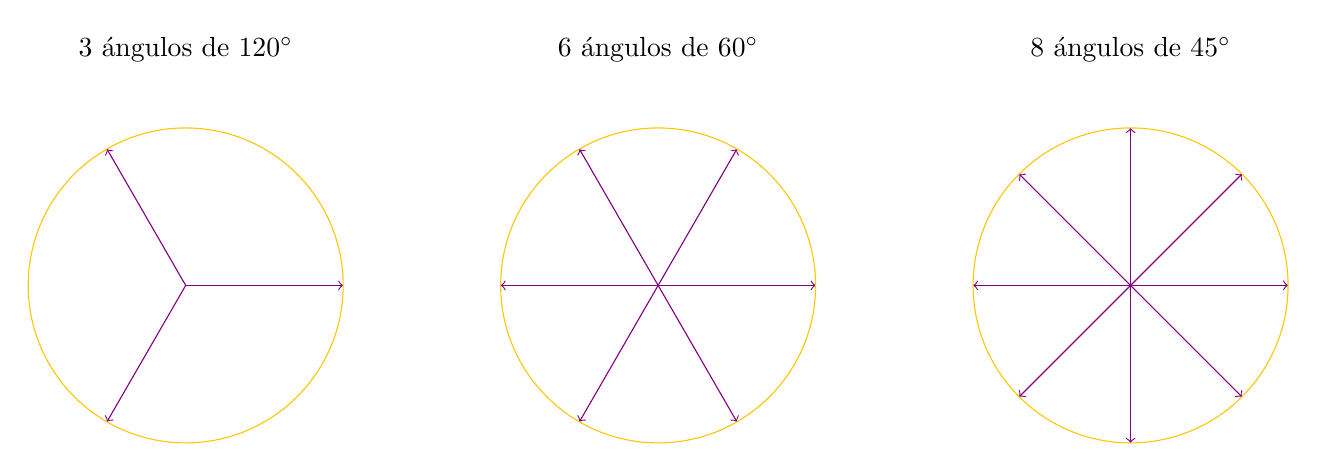
\begin{tikzpicture}
  \draw[arrows=->,color=blue!50!red] (-6,0) -- ++ (120:2);
  \draw[arrows=->,color=blue!50!red] (-6,0) -- ++(0:2);
  \draw[arrows=->,color=blue!50!red] (-6,0) -- ++ (-120:2);
  \node at (-6,3) {3 ángulos de $120^\circ$};
  \draw[color=yellow!80!red] (-6,0) circle[radius=2];

  \draw[arrows=->,color=blue!50!red] (0,0) -- ++ (120:2);
  \draw[arrows=->,color=blue!50!red] (0,0) -- ++(0:2);
  \draw[arrows=->,color=blue!50!red] (0,0) -- ++ (-120:2);
  \draw[arrows=->,color=blue!50!red] (0,0) -- ++ (60:2);
  \draw[arrows=->,color=blue!50!red] (0,0) -- ++(-60:2);
  \draw[arrows=->,color=blue!50!red] (0,0) -- ++ (180:2);
  \node at (0,3) {6 ángulos de $60^\circ$};
  \draw[color=yellow!80!red] (0,0) circle[radius=2];

  
  \draw[arrows=->,color=blue!50!red] (6,0) -- ++ (90:2);
  \draw[arrows=->,color=blue!50!red] (6,0) -- ++(0:2);
  \draw[arrows=->,color=blue!50!red] (6,0) -- ++ (180:2);
  \draw[arrows=->,color=blue!50!red] (6,0) -- ++ (270:2);
  \draw[arrows=->,color=blue!50!red] (6,0) -- ++ (45:2);
  \draw[arrows=->,color=blue!50!red] (6,0) -- ++(135:2);
  \draw[arrows=->,color=blue!50!red] (6,0) -- ++ (-135:2);
  \draw[arrows=->,color=blue!50!red] (6,0) -- ++ (-45:2);
  \node at (6,3) {8 ángulos de $45^\circ$};
  \draw[color=yellow!80!red] (6,0) circle[radius=2];
\end{tikzpicture}
\end{center}

¿Por qué 360 y no otro número? esta pregunta no tiene respuesta, en realidad 360 es un poco arbitrario, su origen es más bien histórico y se sospecha que se debe a un asunto más bien práctico ya que 360 es un número entero que tiene muchos divisores exactos, lo cual hace más probable que los ángulos que usamos resulten tener una medida en el conjunto de los números enteros, pero no hay razones más fuertes, distintas culturas han definido distintas medidas para la circunferencia\footnote{En ingeniería también se usa el sistema \emph{centecimal}, en el cual la circunferencia completa 400 grados, esta unidad de medida se llama {\bf gradián} y se denota con el super índice $g$.}.

Sin embargo, hay una medida que sí es universal y tiene razones matemáticas profundas que la justifican, y por ello ha sido adoptada por la ciencia internacional como medida oficial para los ángulos: {\bf los radianes}.

Se basa en tomar como medida de la circunferencia a su perímetro... ¿pero de cual circunferencia pues el perímetro depende del radio de ésta? para resolver ese dilema, se usa la circunferencia de radio 1, así la circunferencia completa tiene medida $2\pi$\footnote{El 14 de marzo se celebra el día de $\pi$, ya que los primeros 3 dígitos de $\pi$ son 3,14... bromas internacionales de matemáticos, pero que funcionan para recordar este importante número irracional.}.

Como la medida de la circunferencia completa corresponde a su perímetro, {\bf la medida de cada ángulo corresponderá a la longitud del arco que éste delimita dentro de la circunferencia de radio 1}.

Entonces, para medir un ángulo solo debemos colocar su vértice en el centro de una circunferencia de radio 1, y medir el arco que va de una semi recta a la otra... pero hay dos caminos para ir de una recta a la otra, uno largo y uno corto, uno que va girando a favor de los punteros del reloj y otra que va girando en contra, claramente NO tienen la misma longitud ¿Cuál de los dos arcos consideramos para medir?

Hay que decidirse por uno y ser coherente con ello, y la comunidad internacional ha optado por el camino que va contra los punteros del reloj. 

\begin{center}
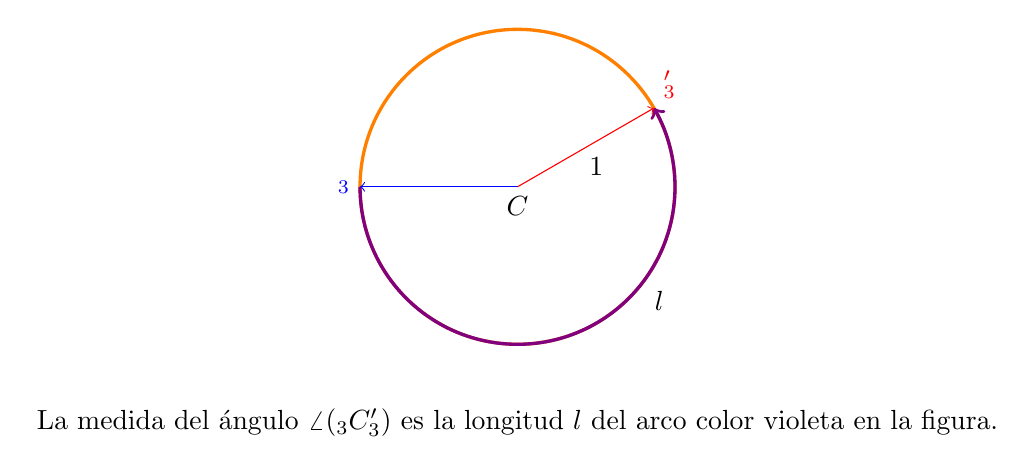
\begin{tikzpicture}
  \coordinate[label=below:$C$] (C) at (6,2);
  \draw[color=orange,very thick] (6,2) circle[radius=2];
  \draw[color=violet, very thick,arrows=->] (4,2) arc[start angle=180, end angle=390,radius=2];
  \draw[arrows=->,color=blue] (6,2) -- ++(-2,0) node[left] {$\calL_3$};
  \draw[arrows=->,color=red] (6,2) -- ++(30:2) node[above right] {$\calL_3'$};
  \coordinate[color=violet,label=below:$l$] (l) at (7.8,0.8);
  \coordinate[label=below:$1$] (r) at (7,2.5);
  \node at (6,-1) {La medida del ángulo $\angle(\calL_3 C \calL_3')$ es la longitud $l$ del arco color violeta en la figura.};
\end{tikzpicture}
\end{center}

Acá el orden toma relevancia, el ángulo $\angle(\calL_3 C \calL_3')$ se mide yendo de $\calL_3$  a $\calL_3'$, por el arco coloreado en violeta.
Por su parte, el ángulo $\angle(\calL_3' C \calL_3)$ se mide por el camino amarillo, pues para ir de $\calL_3'$ a $\calL_3$ contra los punteros del reloj, debemos ir por este arco.
También podemos asignar una medida \emph{negativa} a un ángulo, una medida negativa significa que nos estamos desplazando por la circunferencia a favor de los punteros del reloj.
Con esto, la medida del ángulo $\angle(\calL_3' C \calL_3)$ se puede tomar, de manera equivalente, como el opuesto aditivo de la medida del ángulo $\angle(\calL_3 C \calL_3')$, quedando como $-l$.

Igual que antes, la medida del ángulo corresponde a la porción que representa de la circunferencia completa, solo que en el sistema de radianes esta mide $2\pi$.

\begin{center}
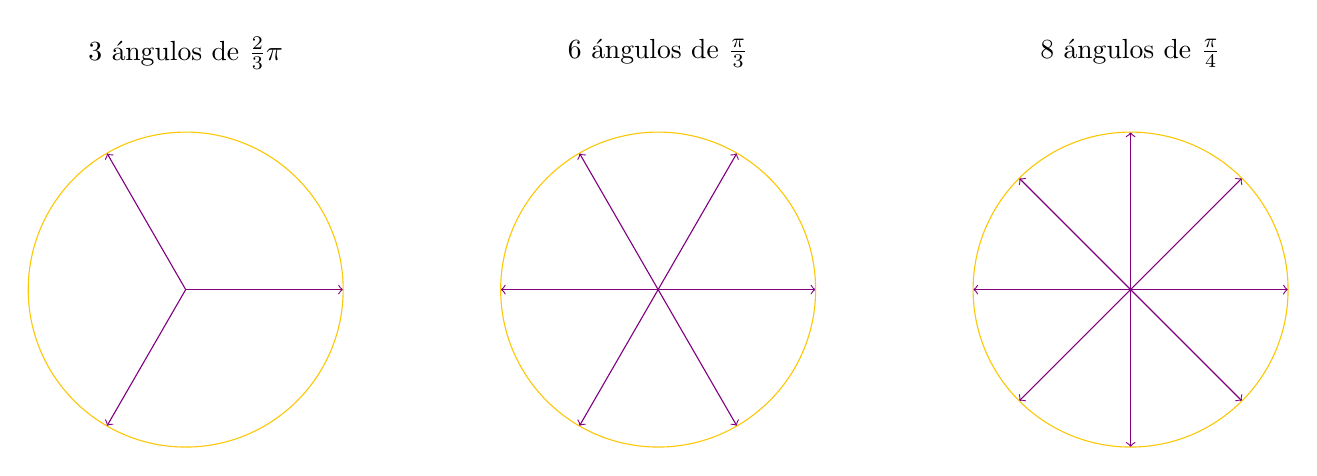
\begin{tikzpicture}
  \draw[arrows=->,color=blue!50!red] (-6,0) -- ++ (120:2);
  \draw[arrows=->,color=blue!50!red] (-6,0) -- ++(0:2);
  \draw[arrows=->,color=blue!50!red] (-6,0) -- ++ (-120:2);
  \node at (-6,3) {3 ángulos de $\frac{2}{3}\pi$};
  \draw[color=yellow!80!red] (-6,0) circle[radius=2];

  \draw[arrows=->,color=blue!50!red] (0,0) -- ++ (120:2);
  \draw[arrows=->,color=blue!50!red] (0,0) -- ++(0:2);
  \draw[arrows=->,color=blue!50!red] (0,0) -- ++ (-120:2);
  \draw[arrows=->,color=blue!50!red] (0,0) -- ++ (60:2);
  \draw[arrows=->,color=blue!50!red] (0,0) -- ++(-60:2);
  \draw[arrows=->,color=blue!50!red] (0,0) -- ++ (180:2);
  \node at (0,3) {6 ángulos de $\frac{\pi}{3}$};
  \draw[color=yellow!80!red] (0,0) circle[radius=2];

  
  \draw[arrows=->,color=blue!50!red] (6,0) -- ++ (90:2);
  \draw[arrows=->,color=blue!50!red] (6,0) -- ++(0:2);
  \draw[arrows=->,color=blue!50!red] (6,0) -- ++ (180:2);
  \draw[arrows=->,color=blue!50!red] (6,0) -- ++ (270:2);
  \draw[arrows=->,color=blue!50!red] (6,0) -- ++ (45:2);
  \draw[arrows=->,color=blue!50!red] (6,0) -- ++(135:2);
  \draw[arrows=->,color=blue!50!red] (6,0) -- ++ (-135:2);
  \draw[arrows=->,color=blue!50!red] (6,0) -- ++ (-45:2);
  \node at (6,3) {8 ángulos de  $\frac{\pi}{4}$};
  \draw[color=yellow!80!red] (6,0) circle[radius=2];
\end{tikzpicture}
\end{center}

En la actualidad, tanto el sistema de grados sexagesimales como el sistema de radianes son muy usados, en particular las coordenadas geográficas de \emph{longitud} y \emph{latitud} de la tierra se miden en grados, pero la ciencia se desarrolla en radianes.

Como en todo sistema de medidas, para pasar de una unidad a otra basta aplicar proporcionalidad, si $g$ es la medida de un ángulo en grados y $r$ su medida en radianes, entonces se cumplirá que $x$ es a $360$ como $r$ es a $2\pi$, lo cual nos provee la siguiente ecuación, que nos servirá en todo momento.

$$\frac{g}{360}=\frac{r}{2\pi}$$

¿Cómo uso ahora la medida de un ángulo para calcular distancias, alturas, areas, etc...? eso lo veremos en la siguiente sección.

\section{Funciones trigonométricas}

¿Para qué nos sirve medir los ángulos? sirve para clasificarlos, para compararlos, para sumarlos... pero ¿para qué más?
De alguna manera un ángulo describe una localización aproximada, nos habla de la dirección (de un objeto por ejemplo), pero si además conocemos la distancia, ya podemos localizar completamente el objeto.

\begin{center}
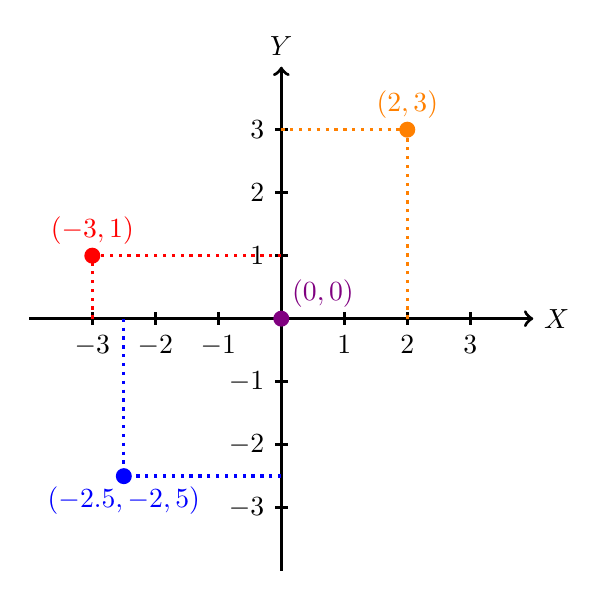
\begin{tikzpicture}[scale=.8,very thick]
\draw[arrows=->] (-4,0) -- (4,0) node[right] {$X$};
\draw[arrows=->] (0,-4) -- (0,4) node[above] {$Y$};
 \foreach \pos in {-3,-2,-1,1,2,3}
    \draw[shift={(\pos,0)}] (0,.1) -- (0,-.1) node[below] {$\pos$};
 \foreach \pos in {-3,-2,-1,1,2,3}
    \draw[shift={(0,\pos)}] (.1,0) -- (-.1,0) node[left] {$\pos$};
\draw[violet,fill=violet] (0,0) circle[radius=0.1] node[above right] {$(0,0)$};
\draw[orange,fill=orange] (2,3) circle[radius=0.1] node[above] {$(2,3)$};
\draw[blue,fill=blue] (-2.5,-2.5) circle[radius=0.1] node[below] {$(-2.5,-2,5)$};
\draw[red,fill=red] (-3,1) circle[radius=0.1] node[above] {$(-3,1)$};
\draw[dotted,orange] (0,3) -- (2,3);
\draw[dotted,orange] (2,0) -- (2,3);
\draw[dotted,blue] (0,-2.5) -- (-2.5,-2.5);
\draw[dotted,blue] (-2.5,0) -- (-2.5,-2.5);
\draw[dotted,red] (0,1) -- (-3,1);
\draw[dotted,red] (-3,0) -- (-3,1);
\end{tikzpicture}
\end{center}

El sistema que más se usa para describir la posición de los objetos es el sistema cartesiano, introducido en el siglo XVII, consiste en definir ejes coordenados perpendiculares (el eje $X$ y el eje $Y$), y describir una posición como un par ordenado $(x,y)$, que indica que para llegar al punto es necesario desplazarse $x$ unidades en dirección del eje $X$ e $y$ unidades en dirección del eje $Y$, partiendo desde el punto de intersección de los ejes, llamado \emph{origen} ($O$).

De manera análoga, si $\calL$ es la semirecta que está sobre el eje $X$, partiendo del origen $O$, entonces el ángulo $\angle(\calL O \calL')$ junto con la distancia $d$ permiten describir un punto indicando que para llegar a él basta desplazarse $d$ unidades en la dirección de $\calL'$. ¿Cómo relacionamos ambos sistemas de localización?

\begin{center}
\begin{tikzpicture}
\draw[color=yellow!80!red,thick] (0,0) circle[radius=2];
\draw[arrows=->] (-3,0) -- (3,0) node[right] {$X$};
\draw[arrows=->] (0,-3) -- (0,3) node[above] {$Y$};
\coordinate[label=below left:$0$] (O) at (0,0);
\draw[arrows=->,color=blue] (0,0) -- (3,0) node[below] {$\calL$};
\draw[arrows=->,color=red] (0,0) -- (57:3) node[right] {$\calL'$};
\draw[fill=black] (57:2) circle[radius=0.1] node[right] {$(x,y)$};
\coordinate[label=right:$d$] (d) at (57:1);
\draw[dotted] (57:2) -- ({2*cos(57)},0);
\draw[dotted] (57:2) -- (0,{2*sin(57)});
\coordinate[label=below:$x$] (x) at ({2*cos(57)},0);
\coordinate[label=left:$y$] (y) at (0,{2*sin(57)});
\coordinate[label=right:$l$] (l) at (26.5:2);
\end{tikzpicture}
\end{center}

La medida del ángulo $\angle(\calL O \calL')$ es $\frac{l}{d}$, y es muy diferente a la coordenada $y$ del punto, no parecen medidas relacionadas de manera simple, pero parece urgente conocer su relación pues se muestra muy útil.

Por otra parte vemos que en la figura aparece un triángulo rectángulo cuyos lados miden justamente $x$ e $y$ y su hipotenusa mide $d$: el triángulo $O(x,0)(x,y)$.
La geometría del triángulo ha sido largamente estudiada y remitirnos a esta podría ayudarnos.

\subsection{La geometría del triángulo rectángulo}

\begin{center}
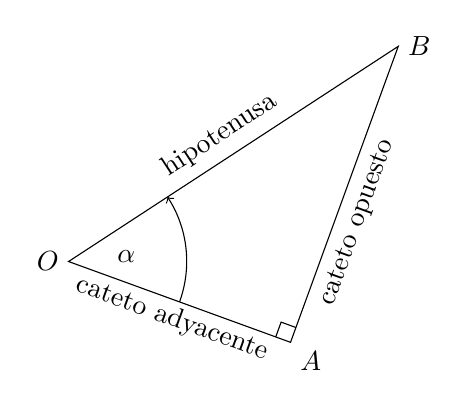
\begin{tikzpicture}
\coordinate[label=left:$O$] (O) at (0,0);
\coordinate[label=below right:$A$] (A) at (-20:3);
\coordinate[label=right:$B$] (B) at (33.13:5);
\draw (O)--(A)--(B)--cycle;
\draw (A)++(160:0.2)-- ++(70:0.2)--++(-20:0.2);
\draw[arrows=<-] (33.13:1.5) arc[start angle=33.13, end angle=-20, radius=1.5];
\coordinate[label=right:$\alpha$] (alpha) at (7.255:.5);
\node[rotate=33.13] at (40:2.5) {hipotenusa};
\node[rotate=-20] at (-29:1.5) {cateto adyacente};
\node[rotate=70] at (7.7:3.7) {cateto opuesto};
\end{tikzpicture}
\end{center}

Un \emph{triángulo} es un polígono de 3 lados.
Tiene 3 vértices y 3 ángulos (de ahí su nombre).

Un \emph{triángulo rectángulo} es un triángulo en que uno de sus ángulos es recto.
Los lados que definen el ángulo recto se llaman \emph{catetos}, mientras que el lado restante se llama \emph{hipotenusa}.

Si tomamos uno de sus ángulos que no es recto  ($\alpha=\angle(A O B)$ en la figura), llamaremos \emph{cateto adyacente} al cateto $AO$ que participa en la definición de $\angle(A O B)$, mientras que el otro cateto se llamará \emph{cateto opuesto}.

Si cambiamos el tamaño de un triángulo sin cambiar sus proporciones obtenemos un triángulo \emph{semejante}.
Los lados de tal triángulo han cambiado, pero no sus relaciones: los cuocientes entre los lados de un triángulo no cambian si escalo el triángulo, tampoco cambian los ángulos. 
Por lo tanto, los cuocientes de las longitudes de sus lados son un invariante bajo escalamiento y nos interesan; no es difícil ver que estas proporciones solo dependen de la medida del ángulo, no de su posición ni orientación,
se definen entonces:
\[
\sen(\alpha)=\frac{\textup{cateto opuesto}}{\textup{hipotenusa}}\qquad \cos(\alpha)=\frac{\textup{cateto adyacente}}{\textup{hipotenusa}}\qquad \tan(\alpha)=\frac{\textup{cateto opuesto}}{\textup{cateto adyacente}}
\]
\begin{center}
\begin{tikzpicture}
\coordinate[label=left:$O$] (O) at (0,0);
\coordinate[label=below right:$A$] (A) at (-20:3);
\coordinate[label=right:$B$] (B) at (33.13:5);
\draw (O)--(A)--(B)--cycle;
\draw (A)++(160:0.2)-- ++(70:0.2)--++(-20:0.2);
\draw[arrows=<-] (33.13:1.5) arc[start angle=33.13, end angle=-20, radius=1.5];
\coordinate[label=right:$\alpha$] (alpha) at (7.255:.5);
\node at (40:2.5) {$h$};
\node at (-29:1.5) {$ca$};
\node at (7.7:3.7) {$co$};
\end{tikzpicture}
\begin{tikzpicture}
\draw[color=white] (0,0)--(1,0);
\end{tikzpicture}
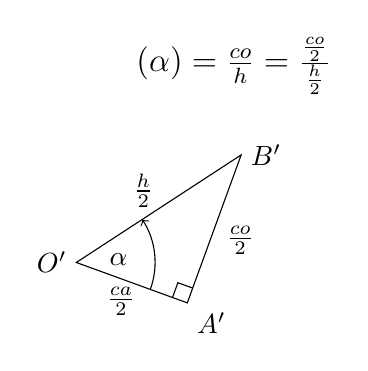
\begin{tikzpicture}
\node at (2,2.5) {{\large $\sen(\alpha)=\frac{co}{h}=\frac{\frac{co}{2}}{\frac{h}{2}}$}};
\coordinate[label=left:$O'$] (O) at (0,0);
\coordinate[label=below right:$A'$] (A) at (-20:3/2);
\coordinate[label=right:$B'$] (B) at (33.13:5/2);
\draw (O)--(A)--(B)--cycle;
\draw (A)++(160:0.2)-- ++(70:0.2)--++(-20:0.2);
\draw[arrows=<-] (33.13:1) arc[start angle=33.13, end angle=-20, radius=1];
\coordinate[label=right:$\alpha$] (alpha) at (7.255:.3);
\node at (47:2.5/2) {$\frac{h}{2}$};
\node at (-41:1.5/2) {$\frac{ca}{2}$};
\node at (7.7:4.2/2) {$\frac{co}{2}$};
\end{tikzpicture}
\end{center}

Estas son las llamadas \emph{funciones trigonométricas}, son estudiadas desde la época de los griegos y resultan tener una relevancia enorme en toda la matemática, tal como verán en Cálculo II y en el resto de su carrera, poseen bellísimas propiedades y se encuentran presentes hasta en los temas más sorprendentes.
No es fácil calcularlas, no tienen una fórmula algebraica, las calculadoras las aproximan usando métodos muy avanzados que ha tomado a la humanidad miles de años descubrir.


¿Qué pasa con el otro ángulo del triángulo rectángulo? Hagamos un poco de teoría para establecer algunas verdades que nos serán útiles.

Lo primero es observar que cuando intersectamos dos rectas cualesquiera se forman 4 ángulos, pero los ángulos que quedan opuestos por un vértice tienen igual medida.

\begin{center}
\begin{tikzpicture}
\draw[name path=L1] (0,0)--++(4,-2) node[below] {$\calL'$};
\draw[name path=L] (0,-2)--++(4,2) node[below] {$\calL$};
\node[name intersections={of=L1 and L},right] at (intersection-1) { $\phantom{m}\alpha$};
\node[name intersections={of=L1 and L},left] at (intersection-1) { $\alpha\phantom{m}$};
\node[name intersections={of=L1 and L},below] at (intersection-1) { $\beta$};
\node[name intersections={of=L1 and L},above] at (intersection-1) { $\beta$};
\end{tikzpicture}
\end{center}

Si ahora agregamos una recta paralela a una de las dos primeras, los ángulos que se forman son los mismos.
Observamos también que los cuatro ángulos suman $2\pi$ y que $\alpha+\beta =\pi$.

\begin{center}
\begin{tikzpicture}
\draw[name path=L1] (0,0)--++(6,-3) node[below] {$\calL'$};
\draw[name path=L2] (3,3)--++(6,-3) node[below] {$\calL''$};
\draw[name path=L] (0,-2)--++(9,4.5) node[below] {$\calL$};
\node[name intersections={of=L1 and L},right] at (intersection-1) { $\phantom{m}\alpha$};
\node[name intersections={of=L2 and L},right] at (intersection-1) { $\phantom{m}\alpha$};
\node[name intersections={of=L1 and L},left] at (intersection-1) { $\alpha\phantom{m}$};
\node[name intersections={of=L2 and L},left] at (intersection-1) { $\alpha\phantom{m}$};
\node[name intersections={of=L1 and L},below] at (intersection-1) { $\beta$};
\node[name intersections={of=L2 and L},below] at (intersection-1) { $\beta$};
\node[name intersections={of=L1 and L},above] at (intersection-1) { $\beta$};
\node[name intersections={of=L2 and L},above] at (intersection-1) { $\beta$};
\end{tikzpicture}
\end{center}


Tomemos ahora tres rectas no paralelas cualesquiera y observemos que se forma un triángulo.
Para aplicar las observaciones anteriores desplazamos una de las rectas paralelamente hasta el otro vértice.
Observamos que $\alpha+\beta+\gamma=\pi$.
Este dibujo se puede repetir para cualquier triángulo, por lo tanto la igualdad que hemos demostrado es verdadera en cualquier triángulo: {\bf la suma de los ángulos interiores de un triángulo es siempre $\pi$ ($180^\circ$)}.

\begin{center}
\begin{tikzpicture}
\draw[name path=Linea 1] (0,-1)--(12,-3) node[below] {$\calL'$};
\draw[name path=Linea 0] (0,-2)--++(8,4) node[below] {$\calL$};
\draw[name path=Linea 2] (5,2)--(8,-4) node[below] {$\calL''$};
\node[name intersections={of=Linea 1 and Linea 0, by=i}, right] at (i) {$\phantom{m}\alpha$};
\draw[name intersections={of=Linea 1 and Linea 2, by=j},color=white] (j) circle(0.2);
\node[rotate=20,above left] at (j) {$\beta$};
\node[name intersections={of=Linea 2 and Linea 0, by=l}, below] at (l) {$\gamma$};
\draw[name path=Linea 3] (l)--++(6,-1) node[below] {$\calL'''$};
\draw (l)--++(-6,1) ;
\node[rotate=20,above left] at (l) {$\beta$};
\node[left] at (i) {$\alpha\phantom{m}$};
\node[left] at (l) {$\alpha\phantom{m}$};
\end{tikzpicture}
\end{center}


¿Cómo se aplica esto a nuestro triángulo rectángulo?


\begin{center}
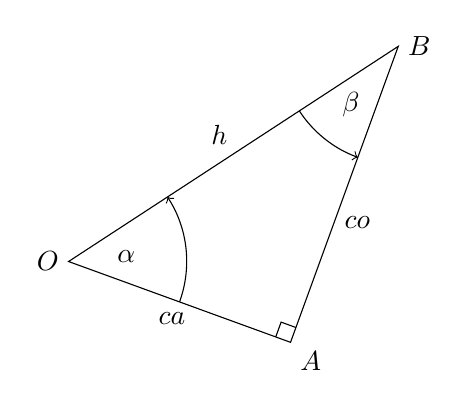
\begin{tikzpicture}
\coordinate[label=left:$O$] (O) at (0,0);
\coordinate[label=below right:$A$] (A) at (-20:3);
\coordinate[label=right:$B$] (B) at (33.13:5);
\draw (O)--(A)--(B)--cycle;
\draw (A)++(160:0.2)-- ++(70:0.2)--++(-20:0.2);
\draw[arrows=<-] (33.13:1.5) arc[start angle=33.13, end angle=-20, radius=1.5];
\coordinate[label=right:$\alpha$] (alpha) at (7.255:.5);
\node at (40:2.5) {$h$};
\node at (-29:1.5) {$ca$};
\node at (7.7:3.7) {$co$};
\node at (29:4.1) {$\beta$};
\draw[arrows=->] (33.13:3.5) arc[start angle=-146.87, end angle=-110, radius=1.5];
\end{tikzpicture}
\end{center}

Los tres ángulos del triángulo de la figura miden: $\alpha$, $\beta$ y $\frac{\pi}{2}$, por lo tanto concluimos que 
$\alpha+\beta+\frac{\pi}{2}=\pi$, de donde se obtiene que:

$$ \alpha+\beta=\frac{\pi}{2}\qquad y \qquad\beta=\frac{\pi}{2}- \alpha$$

De aquí obtenemos las primeras identidades trigonométricas:

 $$\sen\left(\frac{\pi}{2}-\alpha\right)=\cos(\alpha)\qquad \cos\left(\frac{\pi}{2}-\alpha\right)=\sen(\alpha)\qquad \tan\left(\frac{\pi}{2}-\alpha\right)=\frac{1}{\tan(\alpha)}$$

Otra importante identidad se obtiene del {\bf Teorema de Pitágoras}, que afirma que en un triángulo rectángulo se cumple:

$$ ca^2+co^2=h^2$$

No es difícil demostrar este teorema\footnote{De hecho es el teorema matemático con más demostraciones distintas encontradas.}, de manera que no eludiremos ese placer aquí.

\begin{center}
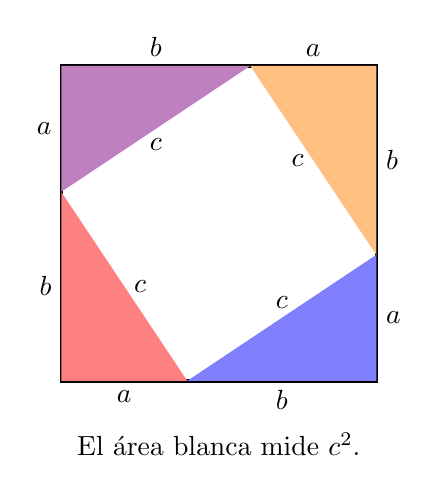
\begin{tikzpicture}[scale=0.4]
\draw[very thick] (0,0)--(10,0)--(10,10)--(0,10)--cycle;
\fill[red!50!white] (0,0)--++(4,0)--++(-4,6)--cycle;
\fill[blue!50!white] (4,0)--++(6,0)--++(0,4)--cycle;
\fill[orange!50!white] (10,4)--++(0,6)--++(-4,0)--cycle;
\fill[violet!50!white] (0,6)--++(6,4)--++(-6,0)--cycle;
\node[below] at (2,0) {$a$};
\node[below] at (7,0) {$b$};
\node[left] at (0,8) {$a$};
\node[left] at (0,3) {$b$};
\node[above] at (8,10) {$a$};
\node[above] at (3,10) {$b$};
\node[right] at (10,2) {$a$};
\node[right] at (10,7) {$b$};
\node[below] at (3,8) {$c$};
\node[above] at (7,2) {$c$};
\node[left] at (8,7) {$c$};
\node[right] at (2,3) {$c$};
\node at (5,-2) {El área blanca mide $c^2$.};
\end{tikzpicture}
\begin{tikzpicture}
\draw[white] (0,0)--(3,0);
\end{tikzpicture}
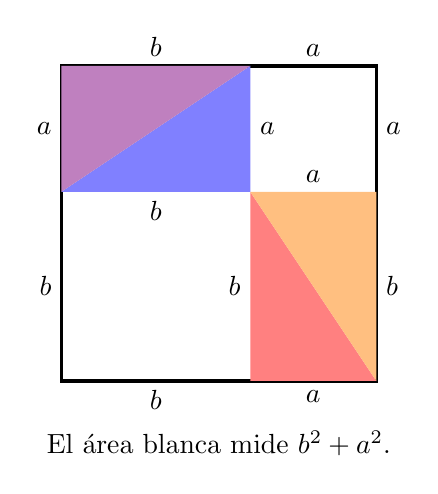
\begin{tikzpicture}[scale=0.4]
\draw[very thick] (0,0)--(10,0)--(10,10)--(0,10)--cycle;
\fill[red!50!white] (6,0)--++(4,0)--++(-4,6)--cycle;
\fill[blue!50!white] (0,6)--++(6,0)--++(0,4)--cycle;
\fill[orange!50!white] (10,0)--++(0,6)--++(-4,0)--cycle;
\fill[violet!50!white] (0,6)--++(6,4)--++(-6,0)--cycle;
\node[below] at (3,0) {$b$};
\node[below] at (8,0) {$a$};
\node[below] at (3,6) {$b$};
\node[above] at (8,6) {$a$};
\node[left] at (0,8) {$a$};
\node[left] at (0,3) {$b$};
\node[right] at (6,8) {$a$};
\node[left] at (6,3) {$b$};
\node[above] at (8,10) {$a$};
\node[above] at (3,10) {$b$};
\node[right] at (10,3) {$b$};
\node[right] at (10,8) {$a$};
\node at (5,-2) {El área blanca mide $b^2+a^2$.};
\end{tikzpicture}
\end{center}

Si dividimos la igualdad dada por el teorema de Pitágoras por la medida de la hipotenusa al cuadrado, obtenemos una identidad muy interesante.

$$ \frac{ca^2+co^2}{h^2}=\frac{h^2}{h^2}\qquad \longrightarrow (\cos(\alpha))^2+(\sen(\alpha))^2=1$$


Las funciones trigonométricas son tremendamente útiles para calcular las dimensiones de un triángulo rectángulo si es que conoces uno de sus ángulos y uno de sus lados, por ejemplo si conoces la hipotenusa, los lados quedan expresados como sigue, pero el ejercicio se puede repetir con los demás lados.

\begin{center}
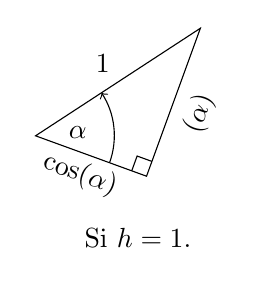
\begin{tikzpicture}
\node at (1.3,-1.3) {Si $h=1$.};
\coordinate (O) at (0,0);
\coordinate (A) at (-20:3/2);
\coordinate (B) at (33.13:5/2);
\draw (O)--(A)--(B)--cycle;
\draw (A)++(160:0.2)-- ++(70:0.2)--++(-20:0.2);
\draw[arrows=<-] (33.13:1) arc[start angle=33.13, end angle=-20, radius=1];
\coordinate[label=right:$\alpha$] (alpha) at (7.255:.3);
\node at (47:2.5/2) {$1$};
\node[rotate=-20] at (-41:1.5/2) {$\cos(\alpha)$};
\node[rotate=70] at (7.7:4.2/2) {$\sen(\alpha)$};
\end{tikzpicture}
\begin{tikzpicture}
\draw[color=white] (0,0)--(3,0);
\end{tikzpicture}
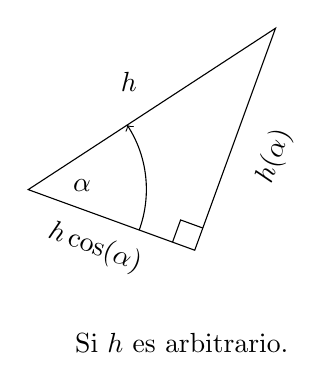
\begin{tikzpicture}[scale=1.5]
\node at (1.3,-1.3) {Si $h$ es arbitrario.};
\coordinate (O) at (0,0);
\coordinate (A) at (-20:3/2);
\coordinate (B) at (33.13:5/2);
\draw (O)--(A)--(B)--cycle;
\draw (A)++(160:0.2)-- ++(70:0.2)--++(-20:0.2);
\draw[arrows=<-] (33.13:1) arc[start angle=33.13, end angle=-20, radius=1];
\coordinate[label=right:$\alpha$] (alpha) at (7.255:.3);
\node at (47:2.5/2) {$h$};
\node[rotate=-20] at (-41:1.5/2) {$h\cos(\alpha)$};
\node[rotate=70] at (7.7:4.2/2) {$h\sen(\alpha)$};
\end{tikzpicture}
\end{center}


Volviendo al problema de la relación entre las coordenadas de un punto especificado por un ángulo, podemos ver que las funciones trigonométricas lo resuelven.


\begin{center}
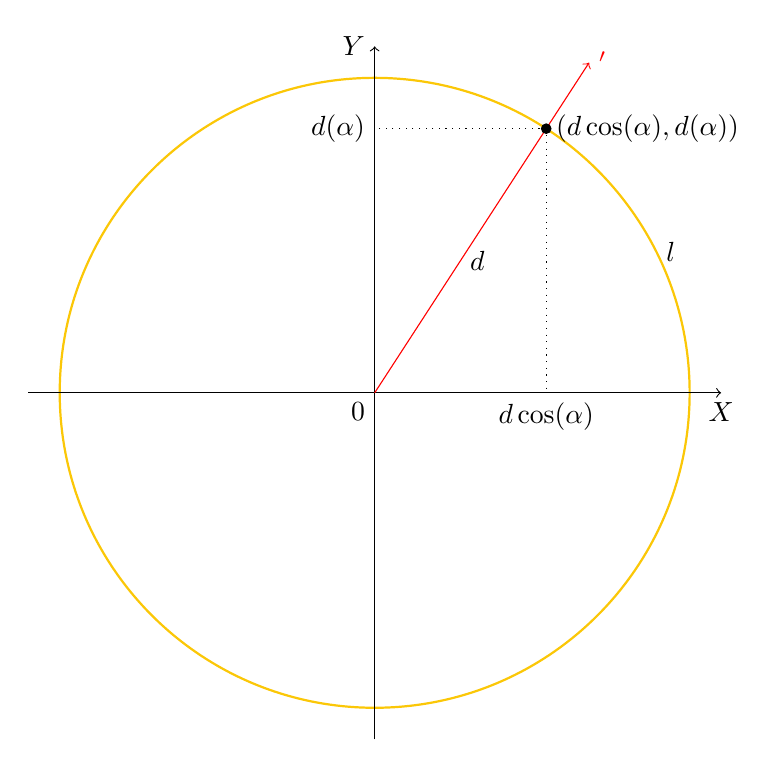
\begin{tikzpicture}[scale=2]
\draw[color=yellow!80!red,thick] (0,0) circle[radius=2];
\draw[arrows=->] (-2.2,0) -- (2.2,0) node[below] {$X$};
\draw[arrows=->] (0,-2.2) -- (0,2.2) node[left] {$Y$};
\coordinate[label=below left:$0$] (O) at (0,0);
\draw[arrows=->,color=red] (0,0) -- (57:2.5) node[right] {$\calL'$};
\draw[fill=black] (57:2) circle[radius=0.03] node[right] {$(d\cos(\alpha),d\sen(\alpha))$};
\coordinate[label=right:$d$] (d) at (57:1);
\draw[dotted] (57:2) -- ({2*cos(57)},0);
\draw[dotted] (57:2) -- (0,{2*sin(57)});
\coordinate[label=below:$d\cos(\alpha)$] (x) at ({2*cos(57)},0);
\coordinate[label=left:$d\sen(\alpha)$] (y) at (0,{2*sin(57)});
\coordinate[label=right:$l$] (l) at (26.5:2);
\end{tikzpicture}
\end{center}

También sirven para calcular un montón de cosas útiles, tales como la altura de un árbol, o el radio de la tierra...

En efecto, en el siglo II antes de Cristo un matemático griego elucubró una técnica para medir el radio de la tierra\footnote{En esos años ya se habían dado cuenta que era esférica.}.
Para hacerlo se valió de una ciudad (Asuán) en la que cierto día del año, a cierta hora caía el sol de manera perpendicular a la tierra, y se reflejaba en el fondo de un pozo.
Sabiendo esto, midió, ese mismo día del año, a esa misma hora, la sombra que producía una torre en otra ciudad lo bastante lejana (Alejandría).
Asumiendo que los rayos del sol llegan con la misma dirección a las dos ciudades (son paralelos), logró calcular una aproximación bastante buena del radio de la tierra.

\begin{center}
\begin{tikzpicture}
\draw[name path=tierra] (0,0) circle(3);
\draw[name path=L1] (0,0)--(31.2:7);
\draw[name path=L2] (0,0)--(24:3);
\draw(0,0)--(24:7) ;
\node[above right] at (25.6:3) {$d$};
\node[below,rotate=24] at (24:3.7) {Asuán};
\node[above,rotate=31.2,align=left] at (31.2:4) {Alejandría};
\node[below,rotate=24] at (24:1.5) {$r$};
\draw(31.2:3)--++(24:4)  node[right] {\phantom{n}sol};
\draw(31.2:3)--++(204:3);
%\draw(0,0)--(24:8);
\end{tikzpicture}
\begin{tikzpicture}
\coordinate[label=right:{Torre}] (t) at (82.8:6);
\draw (-1,0)--(2,0) node(xline) {};
\draw (0,0)--(t)-- (t |-xline) node(b) {};
\node[right] at ($(t)!.5!(b)$) {altura $=t$};
\node[below] at ($(0,0)!.5!(b)$) {sombra $=l$};
\node[left] at ($(t)!.6!(b)$) {$\alpha$};
\draw[arrows=<-] ($(t)!.7!(b)$) arc[start angle=-90, end angle=-97.2,radius=4];
\node at (4,5) {$\tan(\alpha)=\dfrac{l}{t}\sim0.1227$};
\draw[arrows=->] (4,3.5)--(4,2.5);
\node at (4,4) {$\alpha=\dfrac{d}{r}$};
\node at (4,2) {$r=\dfrac{786 [\textup{km}]}{\alpha}$};
\node at (4,1) {$r\sim\dfrac{786 [\textup{km}]}{0.1221}$};
\node at (4,0) {$r\sim6437[\textup{km}]$};
\end{tikzpicture}
\end{center}


\section{Grandes teoremas sobre triángulos}

La semana pasada estudiamos lo que pasaba con el triángulo rectángulo.
Pero la mayoría de los triángulos no son así, necesitamos entonces poder aplicar lo que hemos aprendido a otros triángulos, para lo cual usaremos varias \emph{astucias} y ampliaremos las definiciones de la clase pasada.
\begin{center}
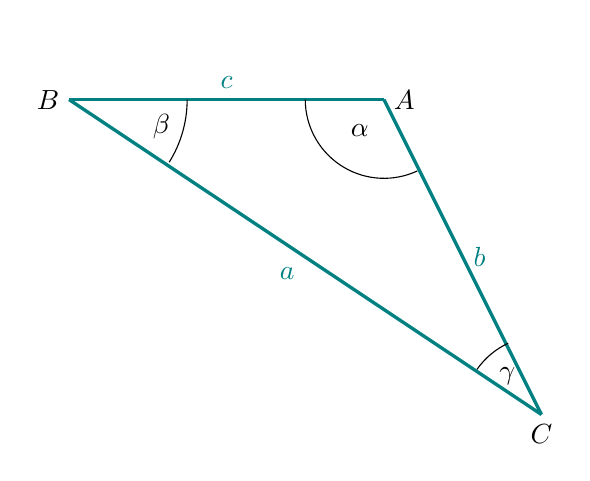
\begin{tikzpicture}[scale=-1]
\coordinate[label=right:$A$] (A) at (0,0);
\coordinate[label=left:$B$](B) at (4,0);
\coordinate[label=below:$C$](C) at (-2,4);
\draw[very thick,green!50!blue] (A)-- node[above] {$c$} (B) node(base) {};
\draw[very thick,green!50!blue] (A)-- node[right] {$b$} (C);
\draw[very thick,green!50!blue] (C)-- node[below left] {$a$} (B);
\coordinate[label=left:$\alpha$] (a) at (80:0.4);
\draw (160:1)++(B) node[right] {$\beta$};
\draw (-30:0.5)++(C) node[above] {$\gamma$};
\draw (0:1) arc[start angle=0, end angle=115,radius=1];
\draw (180:1.5)++(B) arc[start angle=180, end angle=148,radius=1.5];
\draw (-65:1)++(C) arc[start angle=-65, end angle=-35,radius=1];
\end{tikzpicture}
\end{center}
Como vemos, en un triángulo arbitrario pueden haber ángulos mayores que $\frac{\pi}{2}$ (obtusos).
Pero NO puede tener MÁS que UN ángulo mayor que $\frac{\pi}{2}$, ya que los ángulos del triángulo suman $\pi$, tal como vimos la semana pasada.

Sin embargo, las funciones trigonométricas las hemos definido solo para ángulos menores que $\frac{\pi}{2}$ (agudos).
Lo primero que tenemos que hacer es extender nuestra noción de manera conveniente a ángulos obtusos, esto es, ángulos en $[\frac{\pi}{2},\pi]$, y lo hacemos valiéndonos de la circunferencia unitaria y la noción de coordenada.

El ángulo $\angle(X O \calL')$ de medida $\alpha$ en la figura es obtuso.
Definiremos $(\cos(\alpha),\sen(\alpha))$ como las coordenadas $(x,y)$ del punto donde $\calL'$ intersecta a la circunferencia.
La pregunta es ¿cómo calcular estas coordenadas?.
El triángulo rectángulo que se forma lo hemos coloreado en verde, y el ángulo que está en su base mide $\pi-\alpha$, el cual es un ángulo agudo, por lo tanto podemos aplicar las fórmulas vistas en la clase pasada, así: $\sen(\pi-\alpha)=\frac{|y|}{1}=y$, $\textup{cos}(\pi-\alpha)=\frac{|x|}{1}=-x$. 
Por lo tanto, cuando $\alpha\in[\frac{\pi}{2},\pi]$ definimos:
$$\color{blue}{\sen(\alpha)=\sen(\pi-\alpha)}\quad \color{black}{\textup{y}}\quad \color{blue}{\cos(\alpha)=-\cos(\pi-\alpha)}.$$



\begin{center}
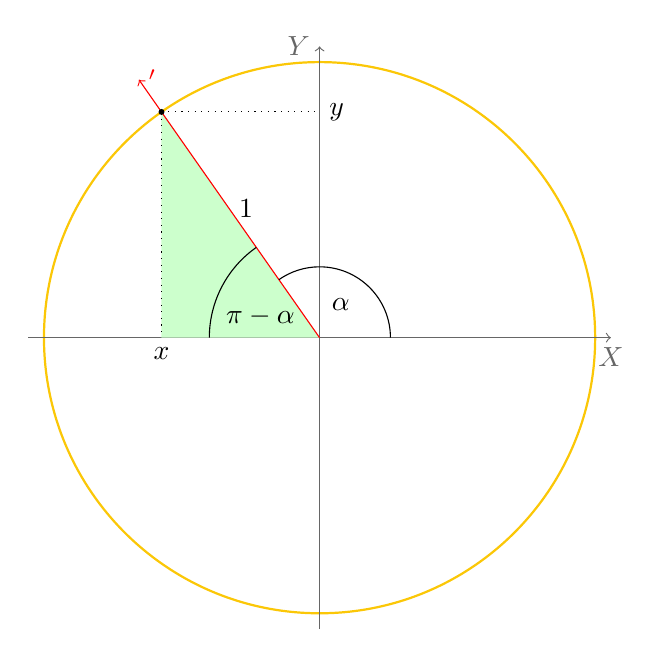
\begin{tikzpicture}
\draw[color=yellow!80!red,thick] (0,0) circle[radius=3.5];
\draw[arrows=->,black!60!white] (-3.7,0) -- (3.7,0) node[below] {$X$};
\draw[arrows=->,black!60!white] (0,-3.7) -- (0,3.7) node[left] {$Y$};

\fill[green!20!white] (0,0)--(125:3.5)--({3.5*cos(125)},0)--cycle;
\draw[arrows=->,color=red] (0,0) -- (125:4) node[right] {$\calL'$};
\draw[fill=black] (125:3.5) circle[radius=0.03] node[right]{}; 
\coordinate[label=right:$1$] (d) at (125:2);
\draw[dotted] (125:3.5) -- ({3.5*cos(125)},0);
\draw[dotted] (125:3.5) -- (0,{3.5*sin(125)});
\coordinate[label=below:$x$] (x) at ({3.5*cos(125)},0);
\coordinate[label=right:$y$] (y) at (0,{3.5*sin(125)});
\coordinate[label=center:$\alpha$] (l) at (57.5:.5);
\draw (.9,0) arc[start angle=0, end angle=125,radius=.9];
\coordinate[label=center:$\pi-\alpha$] (l) at (160:.8);
\draw (-1.4,0) arc[start angle=180, end angle=125,radius=1.4];
\end{tikzpicture}
\begin{tikzpicture}
\draw[white] (0,0)--(1,0);
\end{tikzpicture}
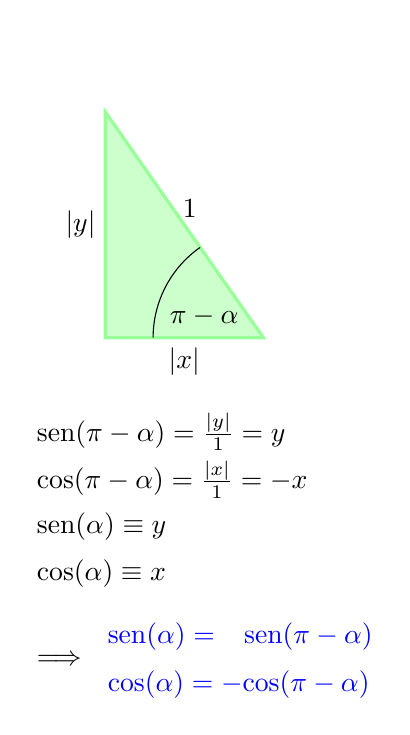
\begin{tikzpicture}
\draw[arrows=->,white] (0,-3.7) -- (0,3.7) node[left] {$Y$};
\fill[green!20!white] (0,0)--(125:3.5)--({3.5*cos(125)},0)--cycle;
\draw[green!40!white,very thick] (0,0)--(125:3.5)--({3.5*cos(125)},0)--cycle;
\coordinate[label=center:$\pi-\alpha$] (l) at (160:.8);
\draw (-1.4,0) arc[start angle=180, end angle=125,radius=1.4];
\coordinate[label=left:$|y|$] (x) at ({3.5*cos(125)},{1.75*sin(125)});
\coordinate[label=below:$|x|$] (y) at ({1.75*cos(125)},0);
\coordinate[label=right:$1$] (d) at (125:2);
\node[right] at (-3,-1.2) {$\textup{sen}(\pi-\alpha)=\frac{|y|}{1}=y$};
\node[right] at (-3,-1.8) {$\textup{cos}(\pi-\alpha)=\frac{|x|}{1}=-x$};
\node[right] at (-3,-2.4) {$\textup{sen}(\alpha)\equiv y$};
\node[right] at (-3,-3) {$\textup{cos}(\alpha)\equiv x$};
\node[right] at (-3,-4.1) {$\Longrightarrow$};
\node[right,blue] at (-2.1,-3.8) {$\textup{sen}(\alpha)=\phantom{-}\textup{sen}(\pi-\alpha)$};
\node[right,blue] at (-2.1,-4.4) {$\textup{cos}(\alpha)=-\textup{cos}(\pi-\alpha)$};
\end{tikzpicture}
\end{center}


\subsection{Teorema del Seno}
\begin{thm}[{\bf del seno}]
Consideremos entonces un tri\'angulo cualquiera $(ABC)$, con lados de longitudes $a$, $b$ y $c$ y \'angulos $\alpha$ (opuesto a lado de longitud $a$), $\beta$ (opuesto a lado de longitud $b$) y $\gamma$ (opuesto a lado de longitud $c$), entonces se cumplen las siguientes igualdades.
\[
\color{blue}{\frac{a}{\sen\alpha} = \frac{b}{\sen\beta} = \frac{c}{\sen\gamma}}
\]
\end{thm}
\begin{proof}
Primero que nada dibujamos el triángulo reposando sobre su lado $AB$.
Hay varios casos, según la forma del triángulo, tal como se ve en la figura siguiente, según $\alpha$, $\beta$ o ninguno sea mayores que $\frac{\pi}{2}$.
El caso en que $\alpha$ es obtuso es análogo al caso en que $\beta$ lo es, de manera que solo analizaremos el caso $\alpha$ obtuso.
\begin{center}
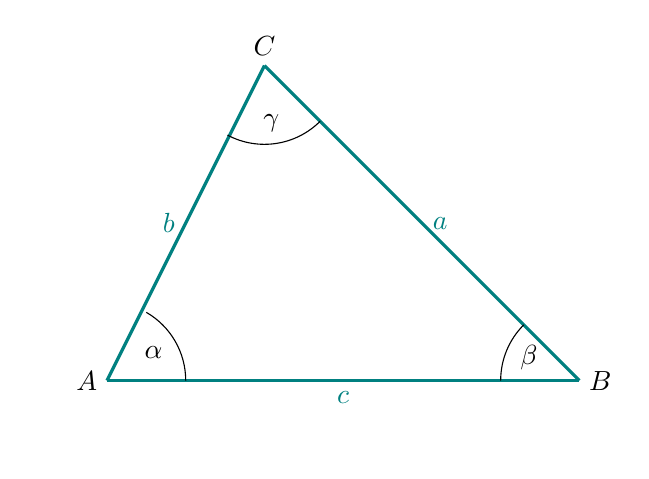
\begin{tikzpicture}
\coordinate[label=left:$A$] (A) at (0,0);
\coordinate[label=right:$B$](B) at (6,0);
\coordinate[label=above:$C$](C) at (2,4);
\draw[very thick,green!50!blue] (A)-- node[below] {$c$} (B) node(base) {};
\draw[very thick,green!50!blue] (A)-- node[left] {$b$} (C);
\draw[very thick,green!50!blue] (C)-- node[right] {$a$} (B);
\coordinate[label=right:$\alpha$] (a) at (45:0.5);
\draw (145:0.5)++(B) node[left] {$\beta$};
\draw (-80:0.5)++(C) node[below] {$\gamma$};
\draw (0:1) arc[start angle=0, end angle=60,radius=1];
\draw (180:1)++(B) arc[start angle=180, end angle=135,radius=1];
\draw (-118:1)++(C) arc[start angle=-118, end angle=-45,radius=1];
\end{tikzpicture}
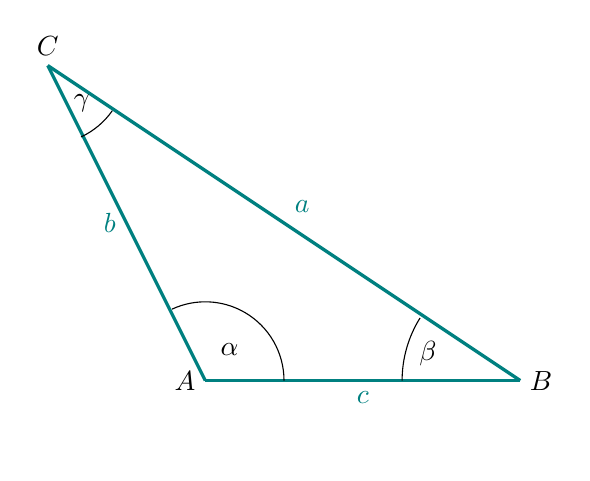
\begin{tikzpicture}
\coordinate[label=left:$A$] (A) at (0,0);
\coordinate[label=right:$B$](B) at (4,0);
\coordinate[label=above:$C$](C) at (-2,4);
\draw[very thick,green!50!blue] (A)-- node[below] {$c$} (B) node(base) {};
\draw[very thick,green!50!blue] (A)-- node[left] {$b$} (C);
\draw[very thick,green!50!blue] (C)-- node[above right] {$a$} (B);
\coordinate[label=right:$\alpha$] (a) at (80:0.4);
\draw (160:1)++(B) node[left] {$\beta$};
\draw (-30:0.5)++(C) node[below] {$\gamma$};
\draw (0:1) arc[start angle=0, end angle=115,radius=1];
\draw (180:1.5)++(B) arc[start angle=180, end angle=148,radius=1.5];
\draw (-65:1)++(C) arc[start angle=-65, end angle=-35,radius=1];
\end{tikzpicture}
\end{center}

Necesitamos triángulos rectángulos para poder aplicar lo que hemos aprendido, entonces trazamos una línea desde $C$ que sea perpendicular al segmento $AB$, y decimos que tiene longitud $h$.	
\begin{center}
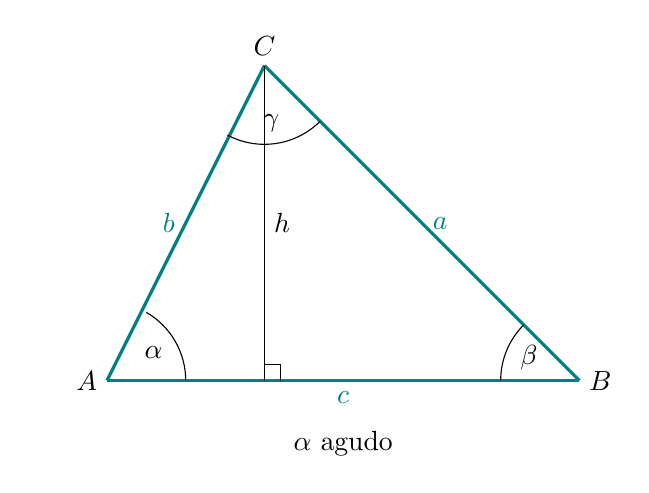
\begin{tikzpicture}
\coordinate[label=left:$A$] (A) at (0,0);
\coordinate[label=right:$B$](B) at (6,0);
\coordinate[label=above:$C$](C) at (2,4);
\draw[very thick,green!50!blue] (A)-- node[below] {$c$} (B) node(base) {};
\draw[very thick,green!50!blue] (A)-- node[left] {$b$} (C);
\draw[very thick,green!50!blue] (C)-- node[right] {$a$} (B);
\coordinate[label=right:$\alpha$] (a) at (45:0.5);
\draw (145:0.5)++(B) node[left] {$\beta$};
\draw (-80:0.5)++(C) node[below] {$\gamma$};
\draw (0:1) arc[start angle=0, end angle=60,radius=1];
\draw (180:1)++(B) arc[start angle=180, end angle=135,radius=1];
\draw (-118:1)++(C) arc[start angle=-118, end angle=-45,radius=1];
\draw (C)-- node[right] {$h$} (C|-base);
\draw (0:0.2)++(C|-base)--++(90:0.2)--++(180:0.2);
\node at (3,-.8) {$\alpha$ agudo};
\end{tikzpicture}
\begin{tikzpicture}
\draw[white] (0,0)--(2.5,0);
\end{tikzpicture}
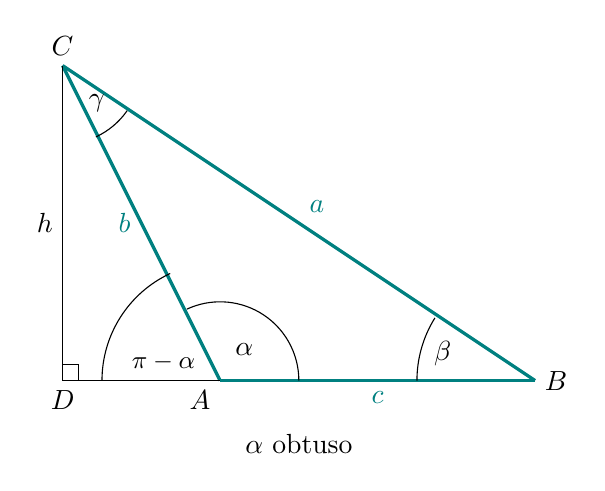
\begin{tikzpicture}
\coordinate[label=below left:$A$] (A) at (0,0);
\coordinate[label=right:$B$](B) at (4,0);
\coordinate[label=above:$C$](C) at (-2,4);
\draw[very thick,green!50!blue] (A)-- node[below] {$c$} (B) node(base) {};
\draw[very thick,green!50!blue] (A)-- node[left] {$b$} (C);
\draw[very thick,green!50!blue] (C)-- node[above right] {$a$} (B);
\coordinate[label=right:$\alpha$] (a) at (80:0.4);
\draw (160:1)++(B) node[left] {$\beta$};
\draw (-30:0.5)++(C) node[below] {$\gamma$};
\draw (0:1) arc[start angle=0, end angle=115,radius=1];
\draw (180:1.5)++(B) arc[start angle=180, end angle=148,radius=1.5];
\draw (-65:1)++(C) arc[start angle=-65, end angle=-35,radius=1];
\draw (C)-- node[left] {$h$} (C|-base);
\draw (0:0.2)++(C|-base)--++(90:0.2)--++(180:0.2);
\draw (C|-base) node[below] {$D$}--(A);
\coordinate[label=left:{\small $\pi-\alpha$}] (d) at (130:0.3);
\draw (180:1.5) arc[start angle=180, end angle=115,radius=1.5];
\node at (1,-.8) {$\alpha$ obtuso};
\end{tikzpicture}
\end{center}

\begin{itemize}
\item[($\alpha$ agudo)]
Entonces usando la definición del seno tenemos lo siguiente.
\[
\sen(\alpha) = \frac h b \dw h = b\sen(\alpha)\;\text{ y }\sen(\beta) = \frac h a \dw h = a\sen(\beta)
\]
Por tanto,
\[
b\sen(\alpha) = a\sen(\beta) \dw \frac{a}{\sen(\alpha)} = \frac{b}{\sen(\beta)}.
\]
\item[($\alpha$ obtuso)]
Nuevamente usamos la definición del seno, pero esta vez sobre el triángulo rectángulo que se forma adyacente al segmento $AC$ por fuera del triángulo.
Aplicando las definiciones establecidas al comienzo de este apunte, tenemos lo siguiente.
\[
\sen(\pi-\alpha) = \frac h b \dw h = \color{magenta}{b\sen(\pi-\alpha)= b\sen(\alpha)}\;\color{black}\text{ y }\sen(\beta) = \frac h a \dw h = a\sen(\beta)
\]
Por tanto,
\[
b\sen(\alpha) = a\sen(\beta) \dw \frac{a}{\sen(\alpha)} = \frac{b}{\sen(\beta)}.
\]
\end{itemize}
Repitiendo esto mismo, pero con la altura sobre otro de los lados del tri\'angulo demostramos el teorema.
\end{proof}	
Este teorema nos dice que existe una proporcionalidad entre los senos de los ángulos y las longitudes de sus segmentos opuestos en un triángulo cualquiera. Por lo tanto es un teorema muy útil para trabajar con triángulos de todo tipo, en especial cuando se conocen más ángulos que lados.
%%%%%%%%%%%%%%%%%%%%%%%%%%%%%%%%%%%%%%%%%%%%%%%%%%%%%%%%


\subsection{Teorema del Coseno}
Tomemos nuevamente el triángulo de la figura y su altura para hacer otro análisis.
Supongamos que esta altura cae en un punto $D$ sobre la recta que contiene al segmento $AB$.
Llamamos $c_1$ a la longitud del segmento $AD$, $c_2$ a la longitud del segmento $DB$ y $c$ a la longitud del segmento $AB$.
Nuevamente el dibujo cambia dependiendo si $\alpha$ es agudo u obtuso.
\begin{center}
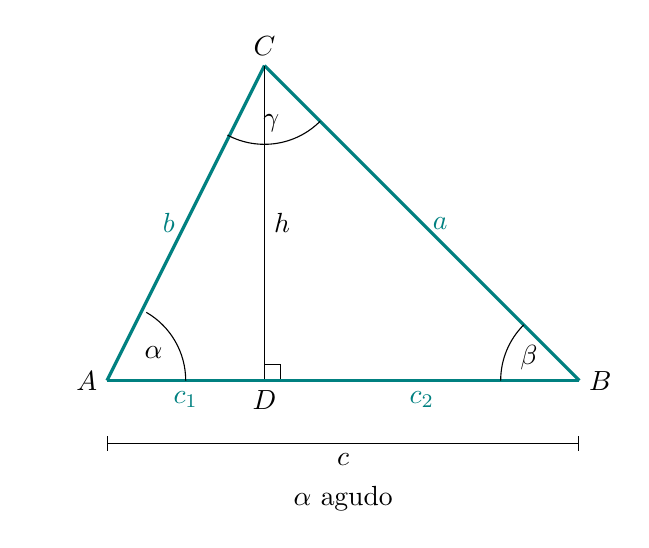
\begin{tikzpicture}
\coordinate[label=left:$A$] (A) at (0,0);
\coordinate[label=right:$B$](B) at (6,0);
\coordinate[label=above:$C$](C) at (2,4);
\draw[very thick,green!50!blue] (A)-- node[below] {} (B) node(base) {};
\draw[very thick,green!50!blue] (A)-- node[left] {$b$} (C);
\draw[very thick,green!50!blue] (C)-- node[right] {$a$} (B);
\coordinate[label=right:$\alpha$] (a) at (45:0.5);
\draw (145:0.5)++(B) node[left] {$\beta$};
\draw (-80:0.5)++(C) node[below] {$\gamma$};
\draw (C)-- node[right] {$h$} (C|-base);
\draw (0:0.2)++(C|-base)--++(90:0.2)--++(180:0.2);
\draw[very thick,green!50!blue] (A)--node[below] {$c_1$} (C|-base);
\draw[very thick,green!50!blue] (B)--node[below] {$c_2$} (C|-base);
\draw[arrows=|-|] (0,-0.8)--node[below] {$c$} (6,-0.8);
\draw (0:1) arc[start angle=0, end angle=60,radius=1];
\draw (180:1)++(B) arc[start angle=180, end angle=135,radius=1];
\draw (-118:1)++(C) arc[start angle=-118, end angle=-45,radius=1];
\node[below] at (C|-base) {$D$};
\node at (3,-1.5) {$\alpha$ agudo};
\end{tikzpicture}
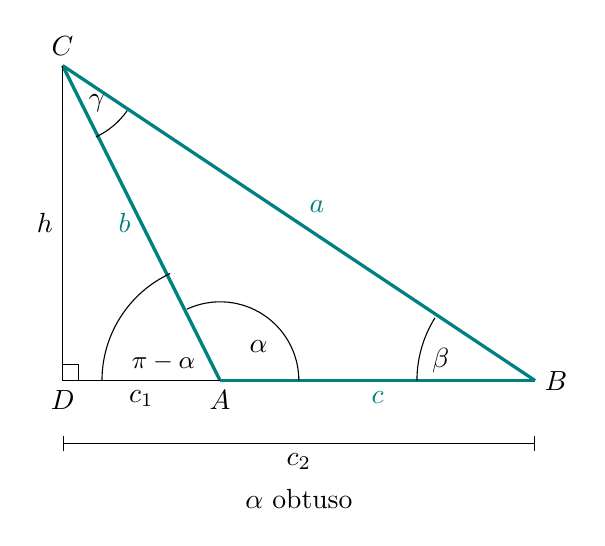
\begin{tikzpicture}
\coordinate[label=below:$A$] (A) at (0,0);
\coordinate[label=right:$B$](B) at (4,0);
\coordinate[label=above:$C$](C) at (-2,4);
\draw[very thick,green!50!blue] (A)-- node[below] {} (B) node(base) {};
\draw[very thick,green!50!blue] (A)-- node[left] {$b$} (C);
\draw[very thick,green!50!blue] (C)-- node[above right] {$a$} (B);
\coordinate[label=right:$\alpha$] (a) at (60:0.5);
\draw (165:1)++(B) node[left] {$\beta$};
\draw (-30:0.5)++(C) node[below] {$\gamma$};
\draw (C)-- node[left] {$h$} (C|-base);
\draw (0:0.2)++(C|-base)--++(90:0.2)--++(180:0.2);
\draw (A)--node[below] {$c_1$} (C|-base); %AD
\draw[very thick,green!50!blue] (B)--node[below] {$c$} (A); %AB
\draw[arrows=|-|] (0,-0.8)++(C|-base)--node[below] {$c_2$} (4,-0.8);

\draw (0:1) arc[start angle=0, end angle=115,radius=1];
\draw (180:1.5)++(B) arc[start angle=180, end angle=148,radius=1.5];
\draw (-65:1)++(C) arc[start angle=-65, end angle=-35,radius=1];

\draw (C|-base) node[below] {$D$}--(A);
\coordinate[label=left:{\small $\pi-\alpha$}] (d) at (130:0.3);
\draw (180:1.5) arc[start angle=180, end angle=115,radius=1.5];
\node at (1,-1.5) {$\alpha$ obtuso};
\end{tikzpicture}
\end{center}
Lo que sigue es una aplicación muy astuta, cuidadosa y conveniente del Teorema de Pitágoras, la definición del coseno y la definición de $c_1$.
Primero, el Teorema de Pitágoras aplicado a los dos triángulos rectángulos adyacentes al segmento $CD$.
\begin{eqnarray}
b^2&=&h^2+c_1^2\label{c1}\quad (\textup{triángulo} (ADC)\label{p1}\\
a^2&=&h^2+c_2^2\label{c2}\quad (\textup{triángulo} (BDC)\label{p2}
\end{eqnarray}
Despejando $h^2$ en (\ref{p1}) y (\ref{p2}) y juntando obtenemos:
\begin{equation}\label{p3}
a^2-c_2^2=b^2- c_1^2\\
\end{equation}
Cuando $\alpha$ es agudo tenemos que $c_1=c-c_2$, mientras que cuando $\alpha$ es obtuso tenemos que $c_1=c_2-c$; en cualquiera de los dos casos se tiene que $c_1^2=(c-c_2)^2=c^2+c_2^2-2cc_2$.
Reemplazando esto en (\ref{p3}) se obtiene lo siguiente.
\begin{eqnarray}\label{p}
a^2-c_2^2&=&b^2-c^2-c_2^2+2cc_2\\
a^2&=&b^2-c^2+2cc_2\\
b^2&=& a^2+c^2-2cc_2\label{p}
\end{eqnarray}
Usamos la definición del coseno sobre el ángulo $\beta$ en el triángulo rectángulo $(BDC)$, y obtenemos lo siguiente.
\[
\cos(\beta) = \frac{c_2}{ a} \dw c_2 = a\cos(\beta)
\]
Reemplazando en (\ref{p}) se concluye que el Teorema del Coseno aplicado al ángulo $\beta$.
$$b^2=a^2+c^2-2ca\cos(\beta)$$
Si repetimos el mismo razonamiento para los demás ángulos, concluimos identidades análogas.
\begin{thm}[{\bf del coseno}]
Consideremos entonces un tri\'angulo cualquiera $(ABC)$, con lados de longitudes $a$, $b$ y $c$ y \'angulos $\alpha$ (opuesto a lado de longitud $a$), $\beta$ (opuesto a lado de longitud $b$) y $\gamma$ (opuesto a lado de longitud $c$), entonces se cumplen las siguientes igualdades.
\begin{eqnarray*}
\color{blue}{a^2}&\color{blue}=&\color{blue}{b^2+c^2-2bc\cos(\alpha)}\\
\color{blue}{b^2}&\color{blue}=&\color{blue}{a^2+c^2-2ac\cos(\beta)}\\
\color{blue}{c^2}&\color{blue}=&\color{blue}{a^2+b^2-2ab\cos(\gamma)}
\end{eqnarray*}
\end{thm}



\subsection{Aplicaciones}

En los siguientes ejemplos, consideramos que las distancias involucradas son lo suficientemente pequeñas como para que la curvatura de la tierra no afecte las medidas, y podamos aplicar la geometría plana que hemos desarrollado a la superficie de la tierra que es esférica.

\begin{ejemplo}
Desde cierta ciudad costera $A$ se observa, a $10[\textup{km}]$ de $A$ y en direcci\'on N$70^\circ$O, una isla $P$.
Un barco parte desde $A$ en direcci\'on sur y en cierto momento de su traves\'{\i}a se observa desde \'el la misma isla $P$, pero en direcci\'on N$30^\circ$O, ¿qu\'e distancia $d$ ha recorrido el barco hasta ese momento?.
\end{ejemplo}
	
Esta situaci\'on corresponde a la mostrada en la figura siguiente.
\begin{center}
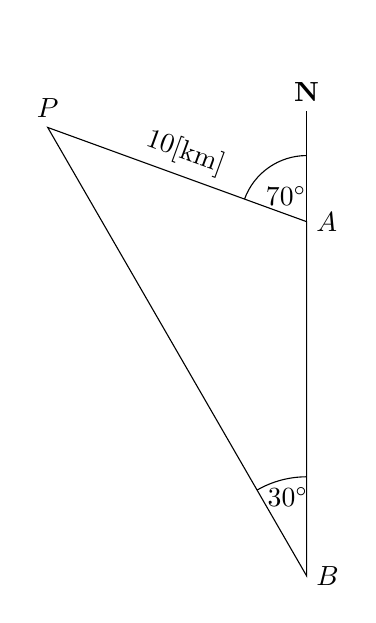
\begin{tikzpicture}[scale=.7]
\coordinate[label=above:$P$](P) at (0,0);
\coordinate[label=right:$A$] (A) at (-20:5);
\coordinate[label=right:$B$] (B) at (-60:9.3969);
\draw (A)--node[above,rotate=-20]{$10[\textup{km}]$}(P)--(B)--cycle;
\draw (A)--++(90:2) node[above] {\bf N};
\draw (90:1.2)++(A) arc[start angle=90, end angle=160,radius=1.2];
\coordinate[label=center:$70^\circ$] (a) at (-16:4.5);
\draw (90:1.8)++(B) arc[start angle=90, end angle=120,radius=1.8];
\coordinate[label=center:$30^\circ$] (a) at (-57:8);
\end{tikzpicture}
\end{center}

				
%		{\bf Variante 1:}
		
		Si denotamos por $\delta$ al \'angulo $BAP$ y por $\gamma$ al \'angulo
		$APB$ se cumple 
		$$\delta = 180^\circ- 70^\circ=110^\circ\quad\textup{y}\quad \gamma + \delta +30^\circ =180^\circ
		\Rightarrow \gamma = 40^\circ,$$
		 con lo que, aplicando el teorema del seno a los ángulos $APB$ y $ABP$ obtenemos
		\[
			\frac{\sen(30^\circ)}{10[\textup{km}]}=\frac{\sen(\gamma)}{d}=\frac{\sen(40^\circ)}{d}.
		\]		
		De donde 
		$$ d=\frac{10\sen(40^\circ)}{\sen(30^\circ)}[\textup{km}]\sim 12,856[\textup{km}]$$
		
		


\begin{ejemplo}
A las 12:00 horas, parten del aeropuerto de Concepci\'on  dos aviones, $A$ y $B$, para rastrear un avi\'on que se precipit\'o al mar.
El Avi\'on $A$ viaja directamente al Oeste a $400[\textup{km}]$ por hora, y el avi\'on $B$ hacia el $N30^{\circ}O$ a $500\textup{km}$ por hora.
A las 14:00 horas el avi\'on $A$ encuentra a los sobrevivientes del avi\'on ca\'ido y llama por radio al avi\'on $B$ para que acuda y ayude en el rescate.
¿A qu\'e distancia est\'a el avi\'on $B$ del avi\'on $A$ en ese momento? 
¿Cu\'anto tiempo demorar\'a el avi\'on $B$ en llegar al rescate?.
\end{ejemplo}	
Consideremos el tri\'angulo $ABC$ con $C$ en el origen, $A$ en el eje 
$X$ y $B$ en el segundo cuadrante (ver figura). 

\begin{center}
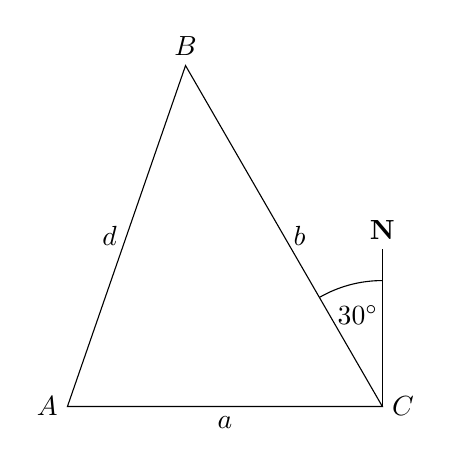
\begin{tikzpicture}[scale=1]
\coordinate[label=above:$B$](B) at (120:5);
\coordinate[label=left:$A$] (A) at (180:4);
\coordinate[label=right:$C$] (C) at (0,0);

\draw (A)--node[below]{$a$}(C)--node[right]{$b$}(B)--node[left]{$d$}cycle;
\draw (C)--++(90:2) node[above] {\bf N};
\draw (90:1.6)++(C) arc[start angle=90, end angle=120,radius=1.6];
\coordinate[label=center:$30^\circ$] (a) at (105:1.2);

\end{tikzpicture}
\end{center}

Como  la velocidad es igual a la distancia dividida por el tiempo y han transcurrido 2 horas, se tiene
$a=2\times400\textup{km}=800\textup{km}$ y $b=2\times500\textup{km}=1000\textup{km}$.

Por otra parte, como el avión $A$ viaja hacia el Oeste, en ángulo $(ACB)$ mide $60^\circ$.

 Por el Teorema del Coseno 
\begin{eqnarray*}
d&=&\sqrt{800^2+1000^2-2\times 800\times 1000\times\cos 60}\textup{km}\\
&=&\sqrt{640.000+1.000.000-1.600.000\times\frac{1}{2}}\textup{km}\\
&=&\sqrt{1.640.000-800.000}\textup{km}\\
&=&\sqrt{840000}\textup{km}\\
&=&100\sqrt{84}\textup{km}
\end{eqnarray*}

Entonces el tiempo que tardará el avión $B$ en llegar al lugar del accidente, suponiendo que mantiene la velocidad (y que puede dar un giro instantáneo sin perder ni un segundo)\footnote{hipótesis muy irrealista, pero necesaria para responder este problema con las herramientas que tenemos.} será de:
\[
t=\frac{d}{v}=\frac{100\sqrt{84}}{500}=\frac{\sqrt{84}}{5}\sim1,8\mbox{ horas.}
\]

\section{Extensión de las funciones trigonométricas a $\R$}


\vspace{.5cm}

Hasta ahora hemos definido las funciones trigonométricas para cualquier ángulo en $[0,\pi]$, pero ¿qué pasa con los demás ángulos? nos interesa definir las funciones en ángulos arbitrarios en $\R$ pues encontramos estos ángulos en el reloj, en una cuerda enrollada a un pilar, en el movimiento rotatorio de los cuerpos, etc.

Consideremos la circunferencia unitaria (centro en origen de coordenadas y radio 1).
Su per\'{\i}metro es igual a $2\pi$.

\begin{center}
\begin{tikzpicture}[scale=2]
\draw[color=yellow!80!red,thick] (0,0) circle[radius=2];
\draw[arrows=->] (-2.2,0) -- (2.2,0) node[below] {$X$};
\draw[arrows=->] (0,-2.2) -- (0,2.2) node[left] {$Y$};
\coordinate[label=below left:$0$] (O) at (0,0);
\coordinate[label=below left:$1$] (x) at (2,0);
\coordinate[label=below left:$-1$]  (x)  at (-2,0);
\coordinate[label=below left:$1$]   (x) at (0,2);
\coordinate[label=below left:$-1$]  (x)  at (0,-2);


\draw[arrows=->,color=red] (0,0) -- (-50:2.5) node[right] {$\calL'$};
\draw[fill=black] (-50:2) circle[radius=0.03] node[right] {$P(l)=(\cos(l),\sen(l))$};
\coordinate[label=right:$1$] (d) at (-50:1);
\draw[dotted] (-50:2) -- ({2*cos(50)},0);
\draw[dotted] (-50:2) -- (0,{-2*sin(50)});
\coordinate[label=below left:$\cos(l)$] (x) at ({2*cos(50)},0);
\coordinate[label=left:$\sen(l)$] (y) at (0,{-2*sin(50)});
\coordinate[label=right:$l$] (l) at (-26.5:2);
\end{tikzpicture}
\end{center}


\begin{defn}
Dado $l\in\R$, definimos el punto $P(l)$ como sigue.
\begin{itemize}
\item Si $l \ge 0$, identificaremos con $P(l)$ al punto sobre la circunferencia unitaria que se obtiene luego de recorrer un arco de longitud $l$ sobre ella comenzando en $(1,0)$ y en sentido anti-horario.

\item Si $l \le 0$, identificaremos con $P(l)$ al punto sobre la circunferencia unitaria que se obtiene luego de recorrer un arco de longitud $|l|$ sobre ella comenzando en $(1,0)$ y en sentido horario.
\end{itemize}
Las coordenadas de $P(l)$ definen las funciones trigonométricas $\sen(l)$ y $\cos(l)$ como aquellos números que cumplen $(\cos(l),\sen(l))=P(l)$.
\end{defn}

\newpage
Los puntos $(1,0)$, $(0,1)$, $(-1,0)$ y $(0,-1)$ en la figura corresponden a $P(0), P\left(\frac{\pi}{2}\right)$, $P(\pi)$ y $P\left(-\frac{\pi}{2}\right)$ respectivamente.
\begin{center}
\begin{tikzpicture}[scale=2]
\draw[color=yellow!80!red,thick] (0,0) circle[radius=2];
\draw[arrows=->] (-2.2,0) -- (2.2,0) node[below] {$X$};
\draw[arrows=->] (0,-2.2) -- (0,2.2) node[left] {$Y$};
\coordinate[label=below left:$0$] (O) at (0,0);
\coordinate[label=below left:$1$] (x) at (2,0);
\coordinate[label=below left:$-1$]  (x)  at (-2,0);
\coordinate[label=below left:$1$]   (x) at (0,2);
\coordinate[label=below left:$-1$]  (x)  at (0,-2);


\draw[fill=black] (0:2) circle[radius=0.05] node[above right] {$P(0)$};
\draw[fill=black] (90:2) circle[radius=0.05] node[above right] {$P(\frac{\pi}{2})$};
\draw[fill=black] (180:2) circle[radius=0.05] node[above left] {$P(\pi)$};
\draw[fill=black] (-90:2) circle[radius=0.05] node[below right] {$P(\frac{\pi}{2})$};
\end{tikzpicture}
\end{center}

Deducimos de esto los siguientes valores para el seno y el coseno.
\begin{enumerate}
	\item $P(0)  = (1,0) \dw \cos(0) = 1, \sen(0) = 0$,
	\item $P\left(\frac{\pi}{2}\right) = (0,1) \dw \cos\left(\frac{\pi}{2}\right) = 0, 
	\sen\left(\frac{\pi}{2}\right) = 1$,
	\item $P(\pi) = (-1,0) \dw \cos(\pi) = -1, \sen(\pi) = 0$,
	\item $ P\left(-\frac{\pi}{2}\right) = (0,-1) \dw 
		 \cos\left(-\frac{\pi}{2}\right) = 0$, $\sen\left(-\frac{\pi}{2}\right) = -1$,
\end{enumerate}



De la definici\'on se desprende adem\'as que cualquiera sea $l\in\R$, se cumple que 
\begin{enumerate}
	\item $\color{blue}{\cos^2(l) + \sen^2(l) = 1}$, tal como vimos en el apunte anterior.
	\item $\color{blue}{ -1 \le \cos(l) \le 1}\color{black}\textup{ y }\color{blue}{ -1 \le \sen (l) \le 1}$, ya que las coordenadas se mantienen dentro de la circunferencia de radio 1.
	\item $\color{blue}{ \cos(l + 2\pi) = \cos(l)}\color{black}\textup{ y }\color{blue}{\sen(l + 2\pi) = \sen(l)}$, pues agregar $2\pi$ solo hace al punto dar una vuelta completa. 

\newpage
	\item $\color{blue}{ \cos(-l) = \cos(l)}\color{black}\textup{ y }\color{blue}{\sen(-l) = -\sen(l)}$, pues tomar el ángulo con signo opuesto equivale a reflejar la figura respecto al eje $X$, se preserva todo pero el signo de la coordenada vertical cambia.
	\item $\color{blue}{ \cos(\pi-l) = -\cos(l)}\color{black}\textup{ y }\color{blue}{\sen(\pi-l) = \sen(l)}$, pues tomar $\pi-l$ en lugar de $l$ es equivalente a tomar el ángulo respecto a la recta opuesta, y medirlo en sentido inverso, es decir, es equivalente a reflejar la figura respecto al eje $Y$.
	\item $\color{blue}{ \cos(l-\frac{\pi}{2}) = \sen(l)}\color{black}\textup{ y }\color{blue}{\sen(l-\frac{\pi}{2}) = -\cos(l)}$, pues restar $\frac{\pi}{2}$ equivale a rotar la figura en $\frac{\pi}{2}$, esto hace que los ejes se intercambien y lo que antes era positivo en la vertical, para a ser negativo en la horizontal.
\end{enumerate}

\begin{center}
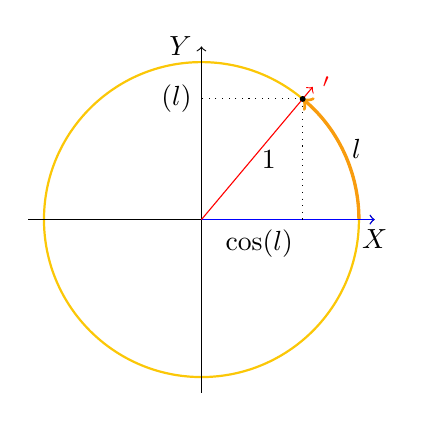
\begin{tikzpicture}[scale=1]
\draw[color=yellow!80!red,thick] (0,0) circle[radius=2];
\draw[arrows=->] (-2.2,0) -- (2.2,0) node[below] {$X$};
\draw[arrows=->] (0,-2.2) -- (0,2.2) node[left] {$Y$};

\draw[arrows=->,color=yellow!60!red,very thick] (2,0) arc[start angle=0, end angle=50,radius=2];
\draw[arrows=->,color=blue] (0,0) -- (2.2,0) node[above] {$\calL$};

\draw[arrows=->,color=red] (0,0) -- (50:2.2) node[right] {$\calL'$};
\draw[fill=black] (50:2) circle[radius=0.03] node[right] {};
\coordinate[label=right:$1$] (d) at (50:1);
\draw[dotted] (50:2) -- ({2*cos(50)},0);
\draw[dotted] (50:2) -- (0,{2*sin(50)});
\coordinate[label=below left:$\cos(l)$] (x) at ({2*cos(50)},0);
\coordinate[label=left:$\sen(l)$] (y) at (0,{2*sin(50)});
\coordinate[label=right:$l$] (-l) at (26.5:2);
\end{tikzpicture}
\begin{tikzpicture}[scale=1]
\draw[white] (-1,-2.2)--(2,2.2); 
\draw[arrows=->] (0,0)--(1,0);
\end{tikzpicture}
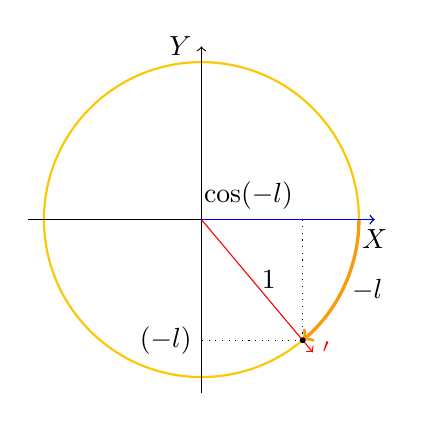
\begin{tikzpicture}[scale=1]
\draw[color=yellow!80!red,thick] (0,0) circle[radius=2];
\draw[arrows=->] (-2.2,0) -- (2.2,0) node[below] {$X$};
\draw[arrows=->] (0,-2.2) -- (0,2.2) node[left] {$Y$};

\draw[arrows=->,color=yellow!60!red,very thick] (2,0) arc[start angle=0, end angle=-50,radius=2];
\draw[arrows=->,color=blue] (0,0) -- (2.2,0) node[above] {$\calL$};

\draw[arrows=->,color=red] (0,0) -- (-50:2.2) node[right] {$\calL'$};
\draw[fill=black] (-50:2) circle[radius=0.03] node[right] {};
\coordinate[label=right:$1$] (d) at (-50:1);
\draw[dotted] (-50:2) -- ({2*cos(50)},0);
\draw[dotted] (-50:2) -- (0,{-2*sin(50)});
\coordinate[label=above left:$\cos(-l)$] (x) at ({2*cos(50)},0);
\coordinate[label=left:$\sen(-l)$] (y) at (0,{-2*sin(50)});
\coordinate[label=right:$-l$] (l) at (-26.5:2);
\end{tikzpicture}
\end{center}

\begin{center}
\begin{tikzpicture}[scale=1]
\draw[white] (-2.2,0)--(2.2,0);
\draw[arrows=->] (0,.5)--(0,-.5);
\end{tikzpicture}
\begin{tikzpicture}[scale=1]
\draw[white] (-1,0)--(2,0); 
\draw[arrows=->] (0,.5)--(1,-.5);
\end{tikzpicture}
\begin{tikzpicture}[scale=1]
\draw[white] (-2.2,0)--(2.2,0);
\end{tikzpicture}
\end{center}

\begin{center}
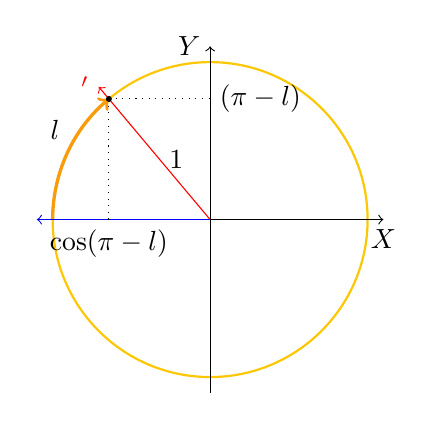
\begin{tikzpicture}[scale=1]
\draw[color=yellow!80!red,thick] (0,0) circle[radius=2];
\draw[arrows=->] (-2.2,0) -- (2.2,0) node[below] {$X$};
\draw[arrows=->] (0,-2.2) -- (0,2.2) node[left] {$Y$};

\draw[arrows=->,color=yellow!60!red,very thick] (-2,0) arc[start angle=180, end angle=130,radius=2];
\draw[arrows=->,color=blue] (0,0) -- (-2.2,0) node[above] {$\calL$};

\draw[arrows=->,color=red] (0,0) -- (130:2.2) node[left] {$\calL'$};
\draw[fill=black] (130:2) circle[radius=0.03] node[right] {};
\coordinate[label=right:$1$] (d) at (130:1);
\draw[dotted] (130:2) -- ({2*cos(130)},0);
\draw[dotted] (130:2) -- (0,{2*sin(130)});
\coordinate[label=below:$\cos(\pi-l)$] (x) at ({2*cos(130)},0);
\coordinate[label=right:$\sen(\pi-l)$] (y) at (0,{2*sin(130)});

\coordinate[label=above left:$l$] (a) at (153.5:2);
\end{tikzpicture}
\begin{tikzpicture}[scale=1]
\draw[white] (-1,-2.2)--(2,2.2); 

\end{tikzpicture}
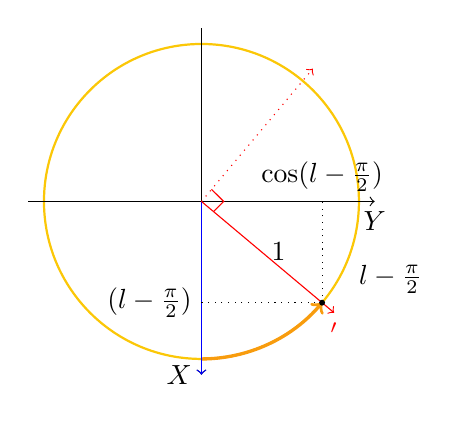
\begin{tikzpicture}[scale=1]
\draw[color=yellow!80!red,thick] (0,0) circle[radius=2];
\draw[arrows=->] (-2.2,0) -- (2.2,0) node[below] {$Y$};
\draw[arrows=->] (0,2.2) -- (0,-2.2) node[left] {$X$};

\draw[arrows=->,color=yellow!60!red,very thick] (0,-2) arc[start angle=-90, end angle=-40,radius=2];
\draw[arrows=->,color=blue] (0,0) -- (0,-2.2) node[right] {$\calL$};

\draw[arrows=->,dotted,color=red] (0,0) -- (50:2.2) node[below] {};
\draw[arrows=->,color=red] (0,0) -- (-40:2.2) node[below] {$\calL'$};
\draw[red] (50:.2)--(0:0.28284)--(-40:.2);
\draw[fill=black] (-40:2) circle[radius=0.03] node[right] {};
\coordinate[label=right:$1$] (d) at (-40:1);
\draw[dotted] (-40:2) -- ({2*cos(-40)},0);
\draw[dotted] (-40:2) -- (0,{2*sin(-40)});
\coordinate[label=above:$\cos(l-\frac{\pi}{2})$] (x) at ({2*cos(-40)},0);
\coordinate[label=left:$\sen(l-\frac{\pi}{2})$] (y) at (0,{2*sin(-40)});
\coordinate[label=below right:$l-\frac{\pi}{2}$] (l) at (-20:2);
\end{tikzpicture}
\end{center}



\newpage 

Podemos graficar la función seno.

\begin{center}
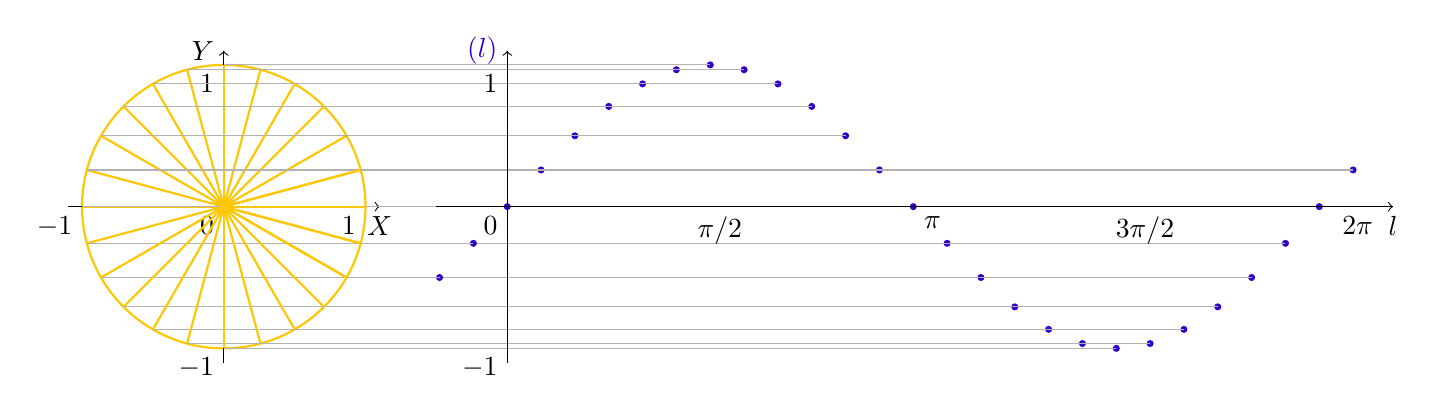
\begin{tikzpicture}[scale=.9]
\draw[color=yellow!80!red,thick] (0,0) circle[radius=2];
\draw[arrows=->] (-2.2,0) -- (2.2,0) node[below] {$X$};
\draw[arrows=->] (0,-2.2) -- (0,2.2) node[left] {$Y$};
\coordinate[label=below left:$0$] (O) at (0,0);
\coordinate[label=below left:$1$] (x) at (2,0);
\coordinate[label=below left:$-1$]  (x)  at (-2,0);
\coordinate[label=below left:$1$]   (x) at (0,2);
\coordinate[label=below left:$-1$]  (x)  at (0,-2);

\foreach \x in {0,...,25} {
\draw[color= yellow!80!red,thick](O)--(15*\x:2);
\fill[color=blue!80!red,thick] (4+0.4774648*\x,{2*sin(15*\x)}) circle[radius=.05];
\draw[black!30!white] (15*\x:2)--(4+0.4774648*\x,{2*sin(15*\x)});
};
\foreach \x in {-1,-2} {
\draw[color= yellow!80!red,thick](O)--(15*\x:2);
\fill[color=blue!80!red,thick] (4+0.4774648*\x,{2*sin(15*\x)}) circle[radius=.05];
\draw[black!30!white] (15*\x:2)--(4+0.4774648*\x,{2*sin(15*\x)});
};
\draw[arrows=->] (3,0) -- (16.5,0) node[below] {$l$};
\draw[arrows=->] (4,-2.2) -- (4,2.2) node[left,blue!80!red] {$\sen(l)$};
\coordinate[label=below left:$0$] (OO) at (4,0);
\coordinate[label=below:$\pi/2$]  (x)  at (7,0);
\coordinate[label=below:$\pi$]  (x)  at (10,0);
\coordinate[label=below:$3\pi/2$]  (x)  at (13,0);
\coordinate[label=below:$2\pi$]  (x)  at (16,0);
\coordinate[label=below left:$1$]   (x) at (4,2);
\coordinate[label=below left:$-1$]  (x)  at (4,-2);

\end{tikzpicture}
\end{center}

¿Cómo son las demás funciones? 

\begin{center}
\begin{tikzpicture}[scale=.9]
\draw[color=yellow!80!red,thick] (0,0) circle[radius=2];
\draw[arrows=->] (-2.2,0) -- (2.2,0) node[below] {$X$};
\draw[arrows=->] (0,-2.2) -- (0,2.2) node[left] {$Y$};
\coordinate[label=below left:$0$] (O) at (0,0);
\coordinate[label=below left:$1$] (x) at (2,0);
\coordinate[label=below left:$-1$]  (x)  at (-2,0);
\coordinate[label=below left:$1$]   (x) at (0,2);
\coordinate[label=below left:$-1$]  (x)  at (0,-2);

\foreach \x in {0,...,25} {
\draw[color= yellow!80!red,thick](O)--(15*\x:2);
\fill[color=blue!60!green,thick] (4+0.4774648*\x  ,{-6+2*cos(15*\x)}) circle[radius=.05];
\draw[black!30!white] (15*\x:2)--({2*cos(15*\x)},{-6+2*cos(15*\x)})--( 4+0.4774648*\x  ,{-6+2*cos(15*\x)});
};
\foreach \x in {-1,-2} {
\draw[color= yellow!80!red,thick](O)--(15*\x:2);
\fill[color=blue!60!green,thick] (4+0.4774648*\x  ,{-6+2*cos(15*\x)}) circle[radius=.05];
\draw[black!30!white] (15*\x:2)--({2*cos(15*\x)},{-6+2*cos(15*\x)})--( 4+0.4774648*\x  ,{-6+2*cos(15*\x)});
};
\draw[arrows=->] (3,-6) -- (16.5,-6) node[below] {$l$};
\draw[arrows=->] (4,-8.2) -- (4,-3.8) node[left,blue!60!green] {$\cos(l)$};
\coordinate[label=below left:$0$] (OO) at (4,-6);
\coordinate[label=below:$\pi/2$]  (x)  at (7,-6);
\coordinate[label=below:$\pi$]  (x)  at (10,-6);
\coordinate[label=below:$3\pi/2$]  (x)  at (13,-6);
\coordinate[label=below:$2\pi$]  (x)  at (16,-6);
\coordinate[label=below left:$1$]   (x) at (4,-4);
\coordinate[label=below left:$-1$]  (x)  at (4,-8);

\end{tikzpicture}
\end{center}


\newpage

¿Y la tangente?

Dado que la circunferencia es unitaria, es decir, la hipotenusa es de longitud 1, entonces, en el triángulo rectángulo con ángulo de medida $l$ en la figura de la circunferencia unitaria se cumple que el cateto opuesto al ángulo mide $\sen(l)$ mientras que el cateto adyacente mide $\cos(l)$, por lo tanto:

\begin{equation}\label{tangente}
\color{blue}{\tan(l)=\frac{\sen(l)}{\cos(l)}}.
\end{equation}

Esta es una buena manera de extender la tangente a los reales, hay que notar sin embargo, que cuando $\cos(l)=0$, la tangente no se podrá definir, y no se le asignará un valor en ese caso.
Pero ese caso corresponde a los ángulos de medida $\pm\pi/2$, es decir los ángulos rectos, lo cual tiene sentido.

Veamos si podemos visualizarla en la circunferencia unitaria, si es que hay algún trazo cuya longitud sea $\tan(l)$.
En realidad la tangente aparece de varias maneras en el diagrama de la circunferencia unitaria.
Primero observamos que $\tan(l)$ es a 1 como $\sen(l)$ es a $\cos(l)$, lo cual es evidente de la ecuación (\ref{tangente}).

$$ \tan(l)=\frac{\tan(l)}{1}=\frac{\sen(l)}{\cos(l)}$$

Esto significa que $\tan(l)$ se puede ver como el cateto opuesto de un triángulo rectángulo con el mismo ángulo $l$, pero con cateto adyacente 1:


\begin{center}
\begin{tikzpicture}[scale=2]

\draw[very thick,green!40!blue] (0,0) -- (2,{2*tan(40)});
\draw[very thick,green!40!blue] (40:2) -- node[left,black] {$\sen(l)$} ({2*cos(40)},0);
\draw[very thick,green!40!blue] (2,0) -- node[right,black] {$\tan(l)$} (2,{2*tan(40)});
\draw[very thick,green!40!blue] (0,0) -- (2,0);
\draw[arrows=|-|] (0,-0.1) -- node[below] {$\cos(l)$} ++({2*cos(40)},0);
\draw[arrows=|-|] (0,-0.5) -- node[below] {$1$} ++(2,0);
\draw[white] (0,0)--(0,-1.8);
\end{tikzpicture}
\begin{tikzpicture}
\draw[white] (0,0)--(1,0);
\end{tikzpicture}
\begin{tikzpicture}[scale=1.5]
\draw[color=yellow!80!red,thick] (0,0) circle[radius=2];
\draw[arrows=->] (-2.2,0) -- (2.2,0) node[below] {$X$};
\draw[arrows=->] (0,-2.2) -- (0,2.2) node[left] {$Y$};

\coordinate[label=below left:$0$] (O) at (0,0);
\coordinate[label=below left:$1$] (x) at (2,0);
\coordinate[label=below left:$-1$]  (x)  at (-2,0);
\coordinate[label=below left:$1$]   (x) at (0,2);
\coordinate[label=below left:$-1$]  (x)  at (0,-2);

\draw[arrows=->,color=red] (0,0) -- (40:3.5) node[right] {$\calL'$};
\draw[fill=black] (40:2) circle[radius=0.03] node[right] {};
\draw[fill=black] (2,{2*tan(40)}) circle[radius=0.03] node[right] {$(1,\tan(l))$};
\coordinate[label=right:$1$] (d) at (40:1);
\draw[dotted] (40:2) -- ({2*cos(40)},0);
\draw[dotted] (2,0) -- (2,{2*tan(40)});
\draw[dotted] (40:2) -- (0,{2*sin(40)});
\coordinate[label=below left:$\cos(l)$] (x) at ({2*cos(40)},0);
\coordinate[label=left:$\sen(l)$] (y) at (0,{2*sin(40)});
\coordinate[label=left:$l$] (l) at (20:2);
\end{tikzpicture}
\end{center}

\newpage

Gracias a esta última observación, podemos graficar la función tangente como sigue.

\begin{center}
\begin{tikzpicture}[scale=.9]
\draw[color=yellow!80!red,thick] (0,0) circle[radius=2];
\draw[arrows=->] (-2.2,0) -- (2.2,0) node[below] {$X$};
\draw[arrows=->] (0,-4) -- (0,4) node[left] {$Y$};
\draw[dotted] (2,-4) -- (2,4);
\draw[dotted] (-2,-4) -- (-2,4);
\coordinate[label=below left:$0$] (O) at (0,0);
\coordinate[label=below left:$1$] (x) at (2,0);
\coordinate[label=below left:$-1$]  (x)  at (-2,0);
\coordinate[label=below left:$1$]   (x) at (0,2);
\coordinate[label=below left:$-1$]  (x)  at (0,-2);

\foreach \x in {5,7,19,17}{
\draw[color= yellow!80!red,thick](O)--(15*\x:4);
};

\foreach \x in {-2,-1,0,1,2,3,4,24,23,22,21,20,25} {
\draw[color= yellow!80!red,thick](O)--(2,{2*tan(15*\x)});
\fill[color=green!10!red,thick] (4+0.4774648*\x,{2*tan(15*\x)}) circle[radius=.05];
\draw[black!30!white] (2,{2*tan(15*\x)})--(4+0.4774648*\x,{2*tan(15*\x)});
};
\foreach \x in {8,9,10,11,12,13,14,15,16} {
\draw[color= yellow!80!red,thick](O)--(-2,{2*tan(15*\x)});
\fill[color=green!10!red,thick] (4+0.4774648*\x,{2*tan(15*\x)}) circle[radius=.05];
\draw[black!30!white] (-2,{2*tan(15*\x)})--(4+0.4774648*\x,{2*tan(15*\x)});
};
\draw[arrows=->] (3,0) -- (16.5,0) node[below] {$l$};
\draw[arrows=->] (4,-4) -- (4,4) node[left,green!10!red] {$\tan(l)$};
\coordinate[label=below left:$0$] (OO) at (4,0);
\fill[white] (7,0) circle[radius=.05];
\fill[white] (13,0) circle[radius=.05];
\coordinate[label=below:$\pi/2$]  (x)  at (7,0);
\coordinate[label=below:$\pi$]  (x)  at (10,0);
\coordinate[label=below:$3\pi/2$]  (x)  at (13,0);
\coordinate[label=below:$2\pi$]  (x)  at (16,0);
\coordinate[label=below:$1$]   (x) at (4,2);
\coordinate[label=below:$-1$]  (x)  at (4,-2);

\end{tikzpicture}
\end{center}

\subsection{Propiedades}


A partir de lo desarrollado en la sección anterior, podemos concluir que los gráficos de las funciones trigonométricas son los siguientes.

\begin{center}
\begin{tikzpicture}
\draw (0,2) node {${\sen(x)}$};
\draw[arrows=->] (-6,0)--(6,0);
\draw[arrows=->] (0,-1.3)--(0,1.3);
\draw[color=red,samples=60,domain=-1.75*pi:1.75*pi]    plot (\x,{sin(\x*360/pi)});
\foreach \y in {pi/2,pi,3*pi/2,2*pi,5*pi/2,3*pi,7*pi/2,-pi/2,-pi,-3*pi/2,-2*pi,-5*pi/2,-3*pi,-7*pi/2}
	\draw (\y/2,-.05)--(\y/2,.05);% node[below] {$\y$};
\node[below] at (pi/4,0) {\small $\frac{\pi}{2}$};
\node[below] at (pi/2,0) {\small $\pi$};
\node[below] at (3*pi/4,0) {\small $\frac{3\pi}{2}$};
\node[below] at (pi,0) {\small $2\pi$};
\node[below] at (5*pi/4,0) {\small $\frac{5\pi}{2}$};
\node[below] at (3*pi/2,0) {\small $3\pi$};
\node[below] at (7*pi/4,0) {\small $\frac{7\pi}{2}$};
\node[below] at (-pi/4,0) {\small $-\frac{\pi}{2}$};
\node[below] at (-pi/2,0) {\small $-\pi$};
\node[below] at (-3*pi/4,0) {\small $-\frac{3\pi}{2}$};
\node[below] at (-pi,0) {\small $-2\pi$};
\node[below] at (-5*pi/4,0) {\small $-\frac{5\pi}{2}$};
\node[below] at (-3*pi/2,0) {\small $-3\pi$};
\node[below] at (-7*pi/4,0) {\small $-\frac{7\pi}{2}$};
\draw (-.05,1)--(.05,1) node[left] {$1$};
\draw (-.05,-1)--(.05,-1) node[left] {$-1$};
\end{tikzpicture}
\end{center}


\begin{center}
\begin{tikzpicture}
\draw (0,2) node {${\cos(x)}$};
\draw[arrows=->] (-6,0)--(6,0);
\draw[arrows=->] (0,-1.3)--(0,1.3);
\draw[color=blue,samples=60,domain=-1.75*pi:1.75*pi]    plot (\x,{cos(\x*360/pi)});
\foreach \y in {pi/2,pi,3*pi/2,2*pi,5*pi/2,3*pi,7*pi/2,-pi/2,-pi,-3*pi/2,-2*pi,-5*pi/2,-3*pi,-7*pi/2}
	\draw (\y/2,-.05)--(\y/2,.05);% node[below] {$\y$};
\node[below] at (pi/4,0) {\small $\frac{\pi}{2}$};
\node[below] at (pi/2,0) {\small $\pi$};
\node[below] at (3*pi/4,0) {\small $\frac{3\pi}{2}$};
\node[below] at (pi,0) {\small $2\pi$};
\node[below] at (5*pi/4,0) {\small $\frac{5\pi}{2}$};
\node[below] at (3*pi/2,0) {\small $3\pi$};
\node[below] at (7*pi/4,0) {\small $\frac{7\pi}{2}$};
\node[below] at (-pi/4,0) {\small $-\frac{\pi}{2}$};
\node[below] at (-pi/2,0) {\small $-\pi$};
\node[below] at (-3*pi/4,0) {\small $-\frac{3\pi}{2}$};
\node[below] at (-pi,0) {\small $-2\pi$};
\node[below] at (-5*pi/4,0) {\small $-\frac{5\pi}{2}$};
\node[below] at (-3*pi/2,0) {\small $-3\pi$};
\node[below] at (-7*pi/4,0) {\small $-\frac{7\pi}{2}$};
\draw (-.05,1)--(.05,1) node[left] {$1$};
\draw (-.05,-1)--(.05,-1) node[left] {$-1$};
\end{tikzpicture}
\end{center}


\begin{center}
\begin{tikzpicture}
\draw (0,5.4) node {${\tan(x)}$};
\draw[arrows=->] (-6,0)--(6,0);
\draw[arrows=->] (0,-5)--(0,5);
%\draw[color=orange,samples=20,domain=-.687:.687]    plot (\x,{tan(\x*360/pi)});
\foreach \y in {pi/2,pi,3*pi/2,2*pi,5*pi/2,3*pi,7*pi/2,-pi/2,-pi,-3*pi/2,-2*pi,-5*pi/2,-3*pi,-7*pi/2}
	\draw (\y/2,-.05)--(\y/2,.05);
\foreach \y in {pi/2,3*pi/2,5*pi/2,7*pi/2,-pi/2,-3*pi/2,-5*pi/2,-7*pi/2}
	\draw[dotted] (\y/2,-5)--(\y/2,5);
\foreach \y in {0,pi/2,pi,3*pi/2,-pi/2,-pi,-3*pi/2}
	\draw[color=orange,samples=20,domain=-.687:.687]    plot (\x+\y,{tan(\x*360/pi)});

\node[below] at (pi/4,0) {\small $\frac{\pi}{2}$};
\node[below] at (pi/2,0) {\small $\pi$};
\node[below] at (3*pi/4,0) {\small $\frac{3\pi}{2}$};
\node[below] at (pi,0) {\small $2\pi$};
\node[below] at (5*pi/4,0) {\small $\frac{5\pi}{2}$};
\node[below] at (3*pi/2,0) {\small $3\pi$};
\node[below] at (7*pi/4,0) {\small $\frac{7\pi}{2}$};
\node[below] at (-pi/4,0) {\small $-\frac{\pi}{2}$};
\node[below] at (-pi/2,0) {\small $-\pi$};
\node[below] at (-3*pi/4,0) {\small $-\frac{3\pi}{2}$};
\node[below] at (-pi,0) {\small $-2\pi$};
\node[below] at (-5*pi/4,0) {\small $-\frac{5\pi}{2}$};
\node[below] at (-3*pi/2,0) {\small $-3\pi$};
\node[below] at (-7*pi/4,0) {\small $-\frac{7\pi}{2}$};
\draw (-.05,1)--(.05,1) node[left] {$1$};
\draw (-.05,-1)--(.05,-1) node[left] {$-1$};
\end{tikzpicture}
\end{center}

Notar que $\tan(\alpha)$ est\'a definida solo si
$\alpha \ne \frac{\pi}{2} + k\pi, \; k \in \Z$, pues son los puntos donde $\cos$ vale 0.

Podemos entonces definir los conjuntos de partida y llegada de las funciones trigonométricas como sigue:

\[
	\sen: \R \To [-1,\,1],\quad \cos: \R \To [-1,\,1],\quad \tan:\R - \left\{\frac{\pi}{2} + k\pi,\;k \in \Z\right\} \To \R
\]

De los gráficos es fácil observar las siguientes propiedades, varias de las cuales ya habían sido demostradas en el capítulo de Trigonometría (apunte TeoremasFunciones.pdf).

\vspace{.2cm}

\begin{prop}
Las funciones trigonométricas tienen las siguientes propiedades como funciones reales.
\begin{enumerate}
\item No son inyectivas.
\item Las funciones seno y coseno tienen periodo $2\pi$.
\item La función tangente tiene periodo $\pi$.
\item Tal como se han definido aquí, son sobreyecivas.
\item Las funciones seno y tangente son impares.
\item La función coseno es par.
\end{enumerate}
\end{prop}

Como vemos, no son biyectivas, pero podemos restringir su conjunto de partida para hacer que lo sean.
Existe una restricción estandarizada, que es la que toman en cuenta la mayor parte de las calculadoras para definir las funciones trigonométricas inversas o ``Arcofunciones''.

\subsection{Inversas de las funciones trigonom\'etricas}

Las restricciones estandarizadas de las funciones trigonométricas son las siguientes.
\begin{itemize}
\item $\sen|_{\left[-\frac{\pi}{2},\frac{\pi}{2}\right]} : \left[-\frac{\pi}{2},\frac{\pi}{2}\right] \To [-1,\,1]$
\item $\cos|_{\left[0,\pi\right]} : \left[0,\pi\right] \To [-1,\,1]$
\item $\tan|_{\left]-\frac{\pi}{2},\frac{\pi}{2}\right[} : \left]-\frac{\pi}{2},\frac{\pi}{2}\right[ \To \R$
\end{itemize}

En las siguientes figuras se muestran, en color fuerte, los grafos correspondientes a estas restricciones, encima de los gráficos de las funciones sin restricción en gris.

\begin{center}
\begin{tikzpicture}
\draw (0,2) node {$\sen(x)|_{[-\frac{\pi}{2},\frac{\pi}{2}]}$};
\draw[white] (0,-5)--(0,5);
\draw[arrows=->] (-1.8,0)--(1.8,0);
\draw[arrows=->] (0,-1.3)--(0,1.3);
\draw[color=white!80!black,samples=20,domain=-pi/2:pi/2]    plot (\x,{sin(\x*360/pi)});
\draw[color=red,samples=20,domain=-pi/4:pi/4,very thick]    plot (\x,{sin(\x*360/pi)});
\foreach \y in {pi/2,-pi/2}
	\draw (\y/2,-.05)--(\y/2,.05);
\node[below] at (pi/4,0) {\small $\frac{\pi}{2}$};
\node[below] at (-pi/4,0) {\small $-\frac{\pi}{2}$};
\draw (-.05,1)--(.05,1) node[left] {$1$};
\draw (-.05,-1)--(.05,-1) node[left] {$-1$};
\fill[red] (pi/4,1) circle (.05);
\fill[red] (-pi/4,-1) circle (.05);
\end{tikzpicture}
\begin{tikzpicture}
\draw[white] (0,0)--(2,0);
\end{tikzpicture}
\begin{tikzpicture}
\draw (0,2) node {$\cos(x)|_{[0,\pi]}$};
\draw[white] (0,-5)--(0,5);
\draw[arrows=->] (-1.8,0)--(1.8,0);
\draw[arrows=->] (0,-1.3)--(0,1.3);
\draw[color=white!80!black,samples=20,domain=-pi/2:pi/2]    plot (\x,{cos(\x*360/pi)});
\draw[color=blue,samples=20,domain=0:pi/2,very thick]    plot (\x,{cos(\x*360/pi)});
\foreach \y in {pi/2,pi}
	\draw (\y/2,-.05)--(\y/2,.05);
\node[below] at (pi/2,0) {\small $\pi$};
\draw (-.05,1)--(.05,1) node[left] {$1$};
\draw (-.05,-1)--(.05,-1) node[left] {$-1$};
\fill[blue] (0,1) circle (.05);
\fill[blue] (pi/2,-1) circle (.05);
\end{tikzpicture}
\begin{tikzpicture}
\draw[white] (0,0)--(2,0);
\end{tikzpicture}
\begin{tikzpicture}
\draw (0,5.4) node {${\tan(x)|_{]-\frac{\pi}{2},\frac{\pi}{2}[}}$};
\draw[arrows=->] (-1.8,0)--(1.8,0);
\draw[arrows=->] (0,-5)--(0,5);
\foreach \y in {pi/2,-pi/2}
	\draw (\y/2,-.05)--(\y/2,.05);

\foreach \y in {-pi/2,pi/2}
	\draw[color=white!80!black,samples=20,domain=-.687:.687]    plot (\x+\y,{tan(\x*360/pi)});
\foreach \y in {0}
	\draw[color=orange,samples=20,domain=-.687:.687,very thick]    plot (\x+\y,{tan(\x*360/pi)});
\node[below] at (pi/4,0) {\small $\frac{\pi}{2}$};
\node[below] at (-pi/4,0) {\small $-\frac{\pi}{2}$};
\draw (-.05,1)--(.05,1) node[left] {$1$};
\draw (-.05,-1)--(.05,-1) node[left] {$-1$};
\end{tikzpicture}
\end{center}

Con estas restricciones definimos las funciones inversas de la siguiente manera.

\begin{defn}		
La inversa de la funci\'on $\sen_{|\left[-\frac{\pi}{2},\frac{\pi}{2}\right]}$ es la función siguiente
\begin{eqnarray*}
	\mbox{Arcsen}: [-1,\,1] &\To& \left[-\frac{\pi}{2},\frac{\pi}{2}\right],\\
	\mbox{Arcsen}(y) = x &\gdw& \sen(x) = y\wedge x \in \left[-\frac{\pi}{2},\frac{\pi}{2}\right]
\end{eqnarray*}
A la inversa de la funci\'on $\cos_{|\left[0,\pi\right]}$ la denotaremos mediante
\begin{eqnarray*}
	\mbox{Arccos}: [-1,\,1] &\To& \left[0,\pi\right],\\
	\mbox{Arccos}(y) = x &\gdw&\cos(x) = y\wedge x \in \left[0,\pi\right]
\end{eqnarray*}
A la inversa de la funci\'on $\tan_{|\left]-\frac{\pi}{2},\frac{\pi}{2}\right[}$ la denotaremos mediante
\begin{eqnarray*}
	\mbox{Arctan}: \R &\To& \left]-\frac{\pi}{2},\frac{\pi}{2}\right[,\\
	\mbox{Arctan}(y) = x &\gdw& \tan(x) = y\wedge x \in \left]-\frac{\pi}{2},\frac{\pi}{2}\right[
\end{eqnarray*}
\end{defn}

Por ejemplo, $\mbox{Arcsen}(0)$ es el \'unico elemento en el intervalo
		$\left[-\frac{\pi}{2},\frac{\pi}{2}\right]$ cuyo seno vale 0, por tanto, $\mbox{Arcsen}(0) = 0$.
		
$\mbox{Arccos}(1)$ es el \'unico elemento en el intervalo $\left[0,\pi\right]$ cuyo coseno vale 1, por tanto, $\mbox{Arccos}(1) = 0$.
		
$\mbox{Arctan}(1)$ es el \'unico n\'umero en $\left]-\frac{\pi}{2},\frac{\pi}{2}\right[$ cuya
		tangente es 1, por tanto, $\mbox{Arctan}(1) = \frac{\pi}{4}$.
		
\begin{center}
\begin{tikzpicture}
\draw (0,2.5) node {$\mbox{Arcsen}(x)|_{[-1,1]}$};
%\draw[white] (0,-5)--(0,5);
\draw[arrows=->] (0,-1.8)--(0,1.8);
\draw[arrows=->] (-1.3,0)--(1.3,0);
\draw[color=red,samples=20,domain=-pi/2:pi/2,very thick]    plot ({sin(\x*180/pi)},\x);
\foreach \y in {pi,pi/2,-pi/2,-pi}
	\draw (-.05,\y/2)--(.05,\y/2);% node[below] {$\y$};
\node[left] at (0,pi/2) {\small $\frac{\pi}{2}$};
\node[left] at (0,-pi/2) {\small $-\frac{\pi}{2}$};
\draw (1,-.05)--(1,.05) node[below] {$1$};
\draw (-1,-.05)--(-1,.05) node[below] {$-1$};
\draw[white] (-1,-1.85)--(-1,-1.75) node[below] {$-1$};
\fill[red] (1,pi/2) circle (.05);
\fill[red] (-1,-pi/2) circle (.05);
\end{tikzpicture}
\begin{tikzpicture}
\draw[white] (0,0)--(2,0);
\end{tikzpicture}
\begin{tikzpicture}
\draw (0,4.3) node {$\mbox{Arccos}(x)|_{[0,\pi]}$};

\draw[arrows=->] (0,0)--(0,3.6);
\draw[arrows=->] (-1.3,0)--(1.3,0);
\draw[color=blue,samples=20,domain=0:pi,very thick]    plot ({cos(\x*180/pi)},\x);
\foreach \y in {pi,pi/2,pi/4,3*pi/4}
	\draw (-.05,\y/2)--(.05,\y/2);
\node[left] at (0,pi/2) {\small $\frac{\pi}{2}$};
\node[left] at (0,pi) {\small $\pi$};
\draw (1,-.05)--(1,.05) node[below] {$1$};
\draw (-1,-.05)--(-1,.05) node[below] {$-1$};
\fill[blue] (1,0) circle (.05);
\fill[blue] (-1,pi) circle (.05);
\end{tikzpicture}
\end{center}

\begin{center}
\begin{tikzpicture}
\draw (0,2.5) node {${\mbox{Arctan}(x)|_{(-\frac{\pi}{2},\frac{\pi}{2})}}$};

\draw[arrows=->] (0,-1.8)--(0,1.8);
\draw[arrows=->] (-5,0)--(5,0);
\foreach \y in {pi,pi/2,-pi/2,-pi}
	\draw (-.05,\y/2)--(.05,\y/2);
\node[left] at (0,pi/2) {\small $\frac{\pi}{2}$};
\node[left] at (0,-pi/2) {\small $-\frac{\pi}{2}$};

\draw[color=orange,samples=20,domain=-1.374:1.374,very thick]    plot ({tan(\x*180/pi)},\x);
 \foreach \pos in {-4,-3,-2,-1,1,2,3,4}
    \draw[shift={(\pos,0)}] (0,.1) -- (0,-.1) node[below] {$\pos$};
\end{tikzpicture}
\end{center}


\begin{ejemplo}
Podemos usar las funciones trigonométricas inversas para resolver ecuaciones que involucren a las funciones trigonométricas o para encontrar ángulos.
\begin{enumerate}
\item $\sen(x) = a$, con $a\in \R$.
		
	Si $a \not \in [-1,1]$ la ecuaci\'on no tiene soluci\'on.
		
	Si $a \in [-1,\,1]$, podemos escribir su conjunto soluci\'on con ayuda de la funci\'on $\mbox{Arcsen}$.
	El n\'umero $\mbox{Arcsen}(a)$ es el \'angulo en $\left[-\frac{\pi}{2},\frac{\pi}{2}\right]$ cuyo seno
	es igual a $a$. Por tanto,
	\[
		S_1 = \left\{\mbox{Arcsen}(a) + 2k\pi\ :\ k \in \Z\right\}
	\]
	est\'a contenido en el conjunto soluci\'on $S$ de la ecuaci\'on dada.
	El \'angulo $\pi-\mbox{Arcsen}(a)$ tambi\'en satisface que su seno es igual a $a$. Por tanto,
	\[
		S = \left\{\mbox{Arcsen}(a) + 2k\pi\ :\ k \in \Z\right\} \cup \left\{\pi-\mbox{Arcsen}(a) + 2k\pi\ :\ k \in \Z\right\}.
	\]			
		
\item $\cos(x) = b$, con $b \in \R$.
		
	Si $b \not \in [-1,1]$ la ecuaci\'on no tiene soluci\'on.
			
	Si $b \in [-1,\,1]$, podemos escribir su conjunto soluci\'on con ayuda de la funci\'on $\mbox{Arccos}$.
	El n\'umero $\mbox{Arccos}(b)$ es el \'angulo en $\left[0,\pi\right]$ cuyo coseno
	es igual a $b$. Por tanto,
	\[
		S_1 = \left\{\mbox{Arccos}(b) + 2k\pi\ :\ k \in \Z\right\}
	\]
	est\'a contenido en el conjunto soluci\'on $S$ de la ecuaci\'on dada.
	El \'angulo $-\mbox{Arccos}(b)$ tambi\'en satisface que su coseno es igual a $b$. Por tanto,
	\[
		S = \left\{\mbox{Arccos}(b) + 2k\pi\ :\ k \in \Z\right\} \cup \left\{-\mbox{Arccos}(b) + 2k\pi\ :\ k \in \Z\right\}.
	\]			
		
\item $\tan(x) = c$, con $c \in \R$.
		
	Esta ecuaci\'on tiene soluci\'on, independientemente del valor de $c$.
	\[
		S = \left\{\mbox{Arctan}(c) + k\pi\ :\ k \in \Z\right\}.
	\]			
\end{enumerate}
\end{ejemplo}


\subsection{Identidades trigonom\'etricas}

Vamos a probar 4 identidades trigonométricas importantes que nos faltó establecer al comienzo del curso, para ello volvemos a mirar la circunferencia unitaria.
\begin{center}
	\resizebox{150mm}{!}{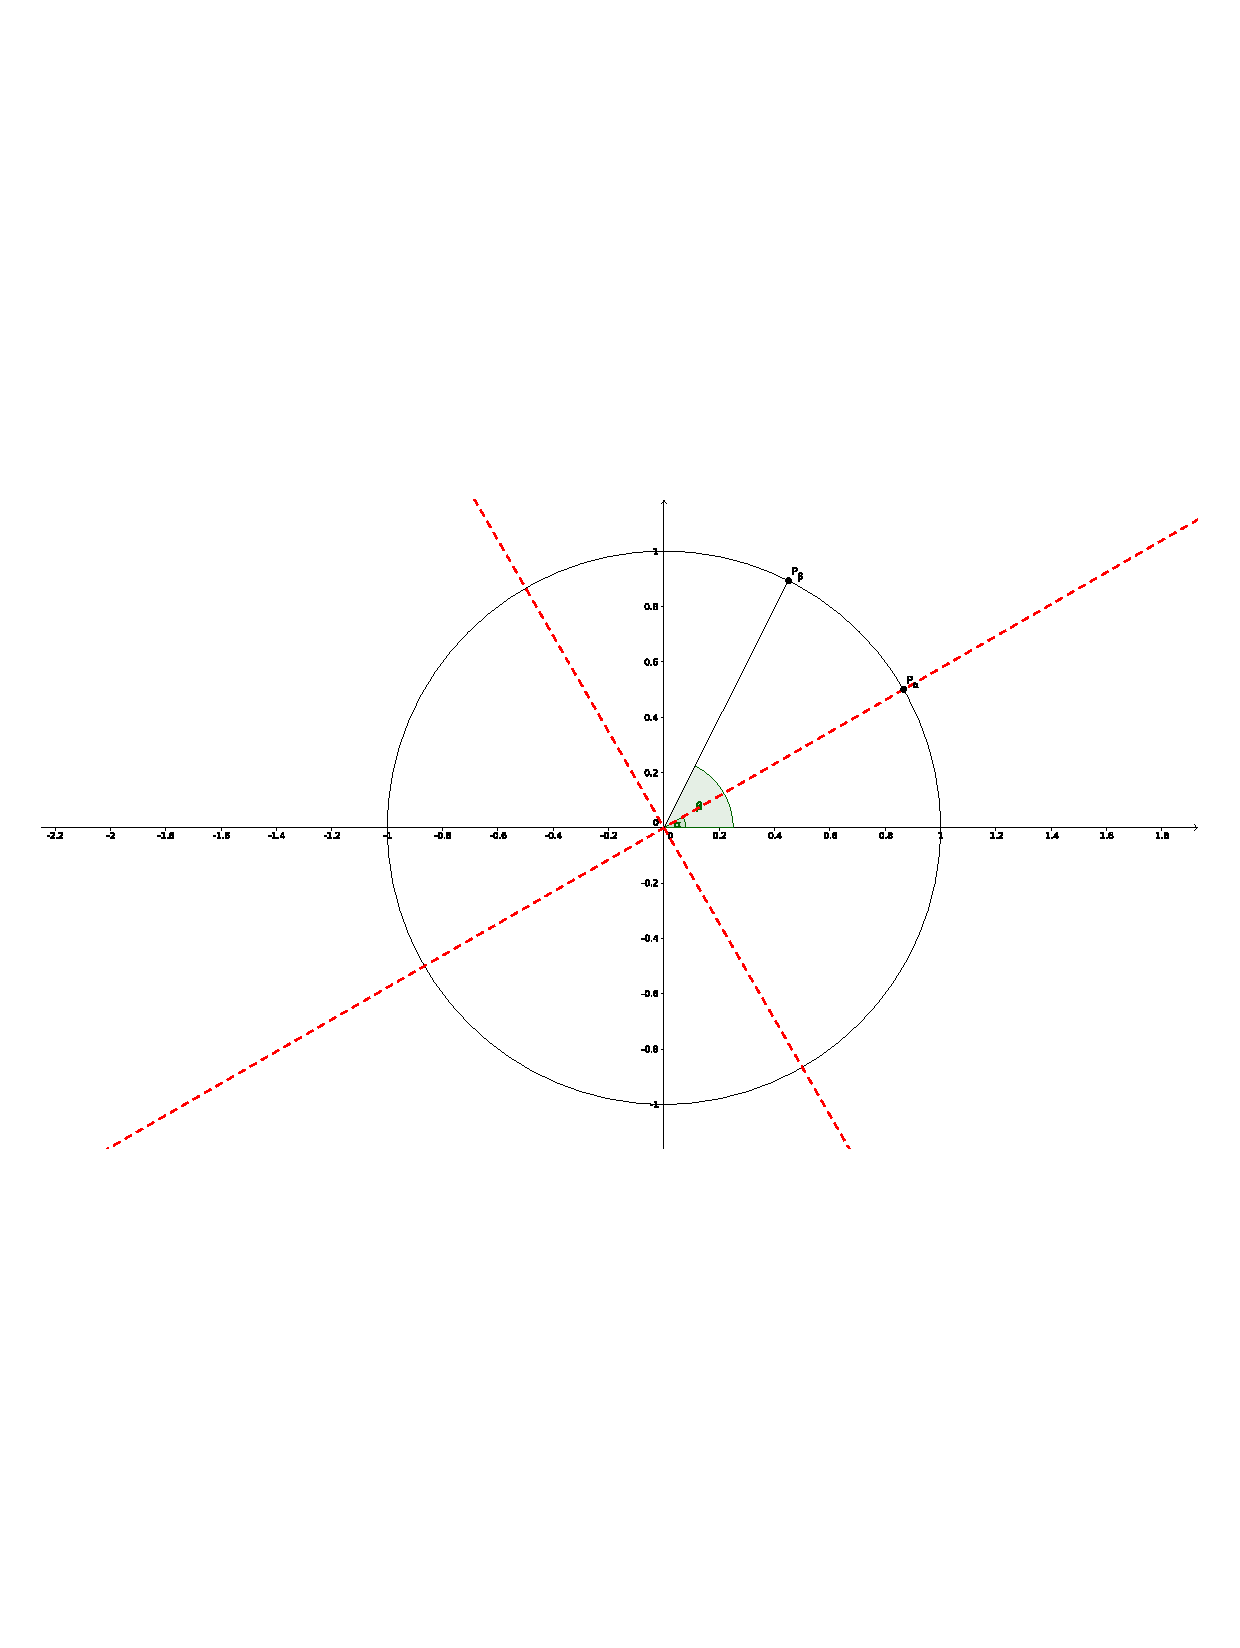
\includegraphics{cos_suma}}
\end{center}
Consideremos $\R^2$ con los ejes cartesianos, pero agreguemos otro par de ejes (en rojo) que corresponden a una rotación de los primeros en un ángulo $\alpha$. 
Las coordenadas del punto $P_{\alpha}$ con respecto a los ejes cartesianos son
$(\cos(\alpha),\sen(\alpha))$, mientras que sus coordenadas con
respecto a los ejes rotados son $(1,0)$.

Consideremos ahora un ángulo $\beta$ (en verde), las coordenadas de $P_{\beta}$ con respecto
a los ejes cartesianos son $(\cos(\beta),\sen(\beta))$ mientras que si se describen con respecto a los
ejes rotados son $(\cos(\beta-\alpha),\sen(\beta-\alpha))$. 

En general, si tomamos dos puntos: $(x_1,y_1)$ y $(x_2,y_2)$, la distancia que los separa se puede obtener por la fórmula:
$$dist((x_1,y_1),(x_2,y_2))=\sqrt{(x_1-x_2)^2+(y_1-y_2)^2}$$
Dado que la distancia entre
dos puntos de un plano no depende de las posiciones de los ejes respecto a los cuales se describen sus coordenadas, tenemos la siguiente igualdad.
\begin{eqnarray*}
 \textrm{medida según los ejes rotados}&=&\textrm{medida según los ejes cartesianos}\\
 (1-\cos(\beta-\alpha))^2 + 
	(0-\sen(\beta-\alpha))^2&=&	(\cos(\alpha)-\cos(\beta))^2 + (\sen(\alpha)-\sen(\beta))^2
\end{eqnarray*}
Si trabajamos esta igualdad, obtenemos lo siguiente.
\begin{eqnarray*}
1-2\cos(\beta-\alpha) + (\cos(\beta-\alpha))^2 + (\sen(\beta-\alpha))^2&=&
	(\cos(\alpha))^2-2\cos(\alpha)\cos(\beta) + (\cos(\beta))^2 +\\
	&& (\sen(\alpha))^2 - 2\sen(\alpha)\sen(\beta) + (\sen(\beta))^2\\
2-2\cos(\beta-\alpha)	-2\cos(\alpha)\cos(\beta) &=&
	  2- 2\sen(\alpha)\sen(\beta)  \\
\cos(\beta-\alpha)&=&\cos(\alpha)\cos(\beta) + \sen(\alpha)\sen(\beta) 
\end{eqnarray*}

\'Esta es una identidad trigonom\'etrica importante, nos da el valor del coseno de la resta de dos \'angulos
$\alpha$ y $\beta$ en t\'erminos de los senos y cosenos de $\alpha$ y $\beta$.

Podemos establecerla como una propiedad, junto con otras más que se desprenden de ella.

\begin{prop}
Dados $\alpha,\beta\in\R$, se cumplen las siguientes propiedades.
\begin{enumerate}
\item $\cos(\beta+\alpha)=\cos(\alpha)\cos(\beta) - \sen(\alpha)\sen(\beta)$
\item $\sen(\alpha + \beta)= \sen(\alpha)\cos(\beta) + \cos(\alpha)\sen(\beta)$
\item $\tan(\alpha + \beta) =  \frac{\tan(\alpha) + \tan(\beta)}{1-\tan(\alpha)\tan(\beta)}$
\item $\cos(2\alpha) = \cos(\alpha+\alpha) = (\cos(\alpha))^2 - (\sen(\alpha))^2$
\item $\sen(2\alpha) = 2\sen(\alpha)\cos(\alpha)$
\item $\tan(2\alpha) = \frac{2\tan(\alpha)}{1-(\tan(\alpha))^2}$
\end{enumerate}
\end{prop}

Las demostraciones se dejan de ejercicio, pero se basan en las identidades trigonométricas que vimos en la primera sección.

